%Alle zu bearbeitenden Felder sind als solche gekennzeichnet. 
%Warnungen sind in der Regel nicht komplett vermeidbar und auch in dieser Vorlage vorhanden (Bei mir 7). Sie sind meistens eher als Hinweise zu verstehen.
%Bei Fragen zu dieser Vorlage einfach eine Mail an gold@lfe.mw.tum.de
%Viel Erfolg!


\documentclass[
	12pt,
	headinclude,
	footinclude,
	a4paper,
	listof=totoc,
	bibliography=totoc,
	index=totoc,
	%twoside, %F�r beidseitigen Druck
	]{scrreprt}


	
	
\newcommand{\myname}[0]{Alfonso Ros and Wahib Ul Haq} %---------- HIER NAME EINTRAGEN ----------
\newcommand{\mythema}[0]{Computer Vision auf mobilen Endger\"aten f\"ur die Ergonomie} %---------- HIER TITEL IN ENGLISCH EINTRAGEN ----------
\newcommand{\mythemaeng}[0]{Computer vision on nomadic devices for human factors engineering} %---------- HIER TITEL EINTRAGEN ----------
\newcommand{\myarbeit}[0]{Interdisciplinary Project} %---------- HIER ART DER ARBEIT EINTRAGEN ----------
\newcommand{\mymodul}[0]{Produktionstechnik} %---------- HIER STUDIENGANGMODUL EINTRAGEN ----------

%----- Bitte au�erdem die Datei _names.tex anpassen ------


\usepackage[
%headinclude, 
%footinclude,
%headsepline,
%footsepline,
%plainfootsepline, 
%plainheadsepline,
automark
]{scrpage2}



\pagestyle{scrheadings}
\clearscrplain
\clearscrheadings
\ofoot[\pagemark]{\pagemark} %Seitenzahlen rechts unten, bitte!
\addtolength{\footskip}{-1cm} %Seitenzahlen ein bisschen h�her setzen


\newcommand{\bild}[4]{
  \begin{figure}[!hbt]
    \begin{center}
    %\centering
      %\vspace{1ex}
      \includegraphics[#2]{img/#1}
      \caption[#4]{\label{img.#1} #3}
    \end{center}
    %\vspace{1ex}
  \end{figure}
 }
 
%bild mit rahmen 
\newcommand{\rbild}[4]{
  \begin{figure}[!hbt]
    \begin{center}
    \fbox{
    %\centering
      %\vspace{1ex}
      \includegraphics[#2]{img/#1}
      }
      \caption[#4]{\label{img.#1} #3}
    \end{center}
    %\vspace{1ex}
  \end{figure}
 }
 
 

\newcommand{\fbild}[5]{
  \begin{floatingfigure}[r]{#5}
    \begin{center}
    %\centering
      %\vspace{1ex}
      \includegraphics[#2]{img/#1}
      \caption[#4]{\label{img.#1} #3}
    \end{center}
    %\vspace{1ex}
  \end{floatingfigure}
 }


\newcommand{\mytab}[4]{
    \begin{table}[!hbt]
    \begin{center}
      \vspace{1ex}
		\begin{tabular}{#2}
			\hline %hline here beacuse hline as first command in included \input-files produces errors
			    \input{tab/#1}
			\hline	    		
		\end{tabular}
          \caption[#4]{\label{tab.#1} #3}
    \end{center}
    \vspace{1ex}
\end{table}
}

\newcommand{\tausend}{\hspace {.5ex}} %50\t 000 => 50 000 tausender trenner 

\newcommand{\comment}[1]{} 

\newcommand{\mytabsmall}[4]{
    \begin{table}[!hbt]
    \begin{center}
      \vspace{1ex}
      {\tiny
		\begin{tabular}{#2}
			\hline %hline here beacuse hline as first command in included \input-files produces errors
			    \input{tab/#1}		
			\hline
		\end{tabular}
		}
          \caption[#4]{\label{tab.#1} #3}
    \end{center}
    \vspace{1ex}
\end{table}
}


% foldersymbol
\newcommand{\folder}[1]{
      \hspace{-3ex}
 \scalebox{0.40}[0.40]
{\includegraphics[viewport=14 15 48 48,clip]{img/folder.pdf}  }
 \bf #1 \normalfont \tiny
 }

% dokumentsymbol 
\newcommand{\dokument}[1]{
      \hspace{-3ex}
 \scalebox{0.60}[0.50]
{\includegraphics[viewport= 22 16 40 42, clip]{img/dokument.pdf}  }
 \bf #1 \normalfont \tiny
 }

% ANWENDUNGSBEISPIELE--------------------------------------------------------------------
%    \bild{meinbild.pdf}{viewport=0 0 200 350, clip=true}{BILDUNTERSCHRIFT}{Eintrag fuers Abbildungsverzeichniss}
%    \bildscale{meinbild.pdf}{viewport=0 0 200 350, clip=true}{BILDUNTERSCHRIFT}{Eintrag fuers 
% 																																									Abbildungsverzeichniss}{scalex}{scaley}
%    \mytab{datei_in_der_die_tabelle_ist.tex}{lrrr <= Format }{TABELLENUNTERSCHRIFT}{Eintrag fuers Tabellenverzeichnis}
%    \dokument[datei$.$mat] % punkt maskieren '$.$' wegen 'dirtree'-umgebung
%    \folder[mydirectory]



% macht den rand schoener (optischer randausgleich)
\usepackage[activate=normal]{pdfcprot}


\usepackage{units}
%\unit[Wert]{Einheit}
%\unitfrac[Wert]{Z�hler}{Nenner}

\newcommand{\myunit}[1]{\,\unit{#1}}  % ohne []
\newcommand{\myunitrm}[1]{\,\mathrm{\unit{#1}}} % mit []
\newcommand{\myunitfrac}[2]{\,\mathrm{\unitfrac{#1}{#2}}}
%
%U = 2.459\, 123 \myunit{V}
%\sigma = \frac{F}{A} = 133.432\, 192\, 233 \myunitfrac{N}{mm^{2}}

\usepackage{url}

\usepackage[plainpages=false,ngerman,pdfpagelabels=true,bookmarks=true, 
						%bookmarksopen=true, % waehrend testen offen lassen spaeter zumachen
						pdfpagemode={UseOutlines},pdfstartview={FitV},pdfborder={0 0 0},
						pdfauthor={\myname}, 
						pdftitle={\mythema},
						%pdfsubject={\mythema}, % optional
						%pdfkeywords={Schluesselwort1,Schluesselwort2,Schluesselwort3},
						colorlinks=true,
						linkcolor=black,
						filecolor=black,
						urlcolor=black,
						citecolor=black,
						hypertexnames=true,
						pdfpagelabels=true,
						hyperindex=true,
						linktocpage=true,
						pagebackref=true
						]{hyperref}
						
						

	\usepackage[round]{natbib}
 
	\usepackage{geometry}
%	\geometry{left=3.5cm,textwidth=15cm,top=2.5cm,textheight=24.5cm}
%	\geometry{left=2.5cm, right=2.5cm, bottom=3cm, top=2.5cm}
	\geometry{left=3cm, right=2.6cm, bottom=3cm, top=2.5cm}
	
	\usepackage{makeidx}
	\makeindex

\usepackage{setspace}
%\onehalfspacing %Zu klein im Vergleich zu Word
\setstretch{1.54} %Simuliert den 1,5 fachen Zeilenabstand von Word (Bei dieser Schriftart und dieser Schriftgr��e)
\renewcommand{\arraystretch}{1.54} %Zeilenabstand in Tabellen! 

\setlength{\parindent}{0pt} %Kein Einr�cken der ersten Zeile eines Absatzes
\setlength{\headheight}{1.1\baselineskip}

\usepackage{titlesec} %Dieser Abschnitt definiert die �berschriften
\titleformat{\chapter}[block]{\large\bfseries}{\thechapter}{.5em}{}
\titleformat{\section}[block]{\large\bfseries}{\thesection}{.5em}{}
\titleformat{\subsection}[block]{\large\bfseries}{\thesubsection}{.5em}{}
\titleformat{\subsubsection}[block]{\large\bfseries}{\thesubsubsection}{.5em}{}

%
%
%\setlength{\headsep}{1cm}
%\setkomafont{pagefoot}{\normalfont} %Sonst wird Fu�zeile kursiv
%\setkomafont{pageheadfoot}{\normalfont} %Sonst wird Kopfzeile kursiv
%
%%\pagestyle{scrheadings}
\clearscrheadfoot % clear header and footer
%\automark[section]{chapter}
%\ihead[]{\leftmark} % header left part
%%\ohead[]{\rightmark} % header right part
%\ohead[]{\scalebox{0.05}{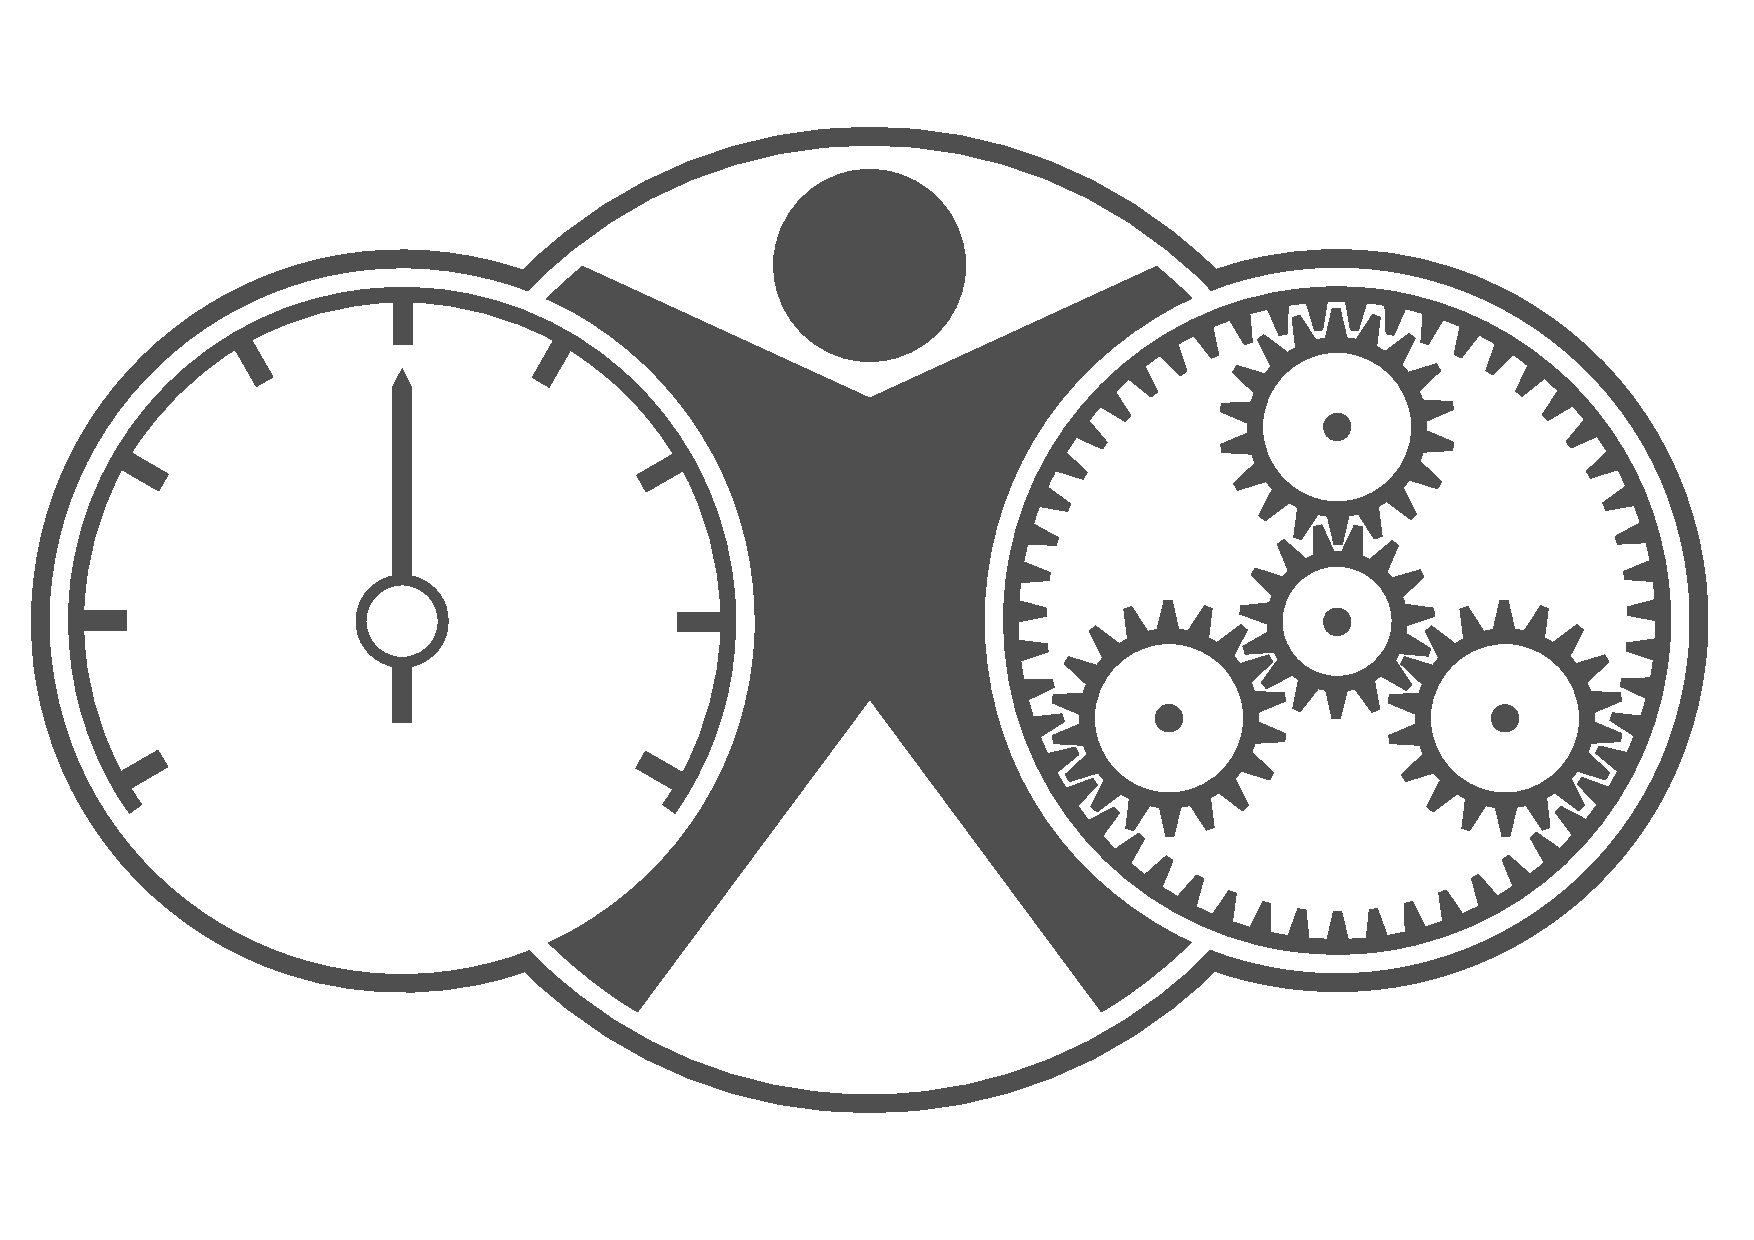
\includegraphics{img/lfe.pdf}}} % header right part
%\ifoot{\small \myarbeit \space \myname} % footer left part  
%%\cfoot{\vspace{-0.5cm}\mythema} % footer middle part
%%\ofoot{Seite\ {\pnumfont \pagemark}\ von {\pnumfont \pageref{LastPage}}} % footer right part
\ofoot{\small {\pnumfont \pagemark}} % footer right part
%\setheadsepline{0.3pt} % set header seperate line
%\setfootsepline{0.3pt} % set footer seperate line
%%\setheadwidth{textwithmarginpar}
%%\setfootwidth{textwithmarginpar}



\usepackage[dvips]{graphicx}
\usepackage{floatflt,epsfig} 

\usepackage{ngerman} % neue deutsche Rechtschreibung
\usepackage[latin1]{inputenc} % latin1-Kodierung f�r Umlaute
\usepackage[ngerman]{babel}  % Silbentrennung
\usepackage[T1]{fontenc}
\usepackage[scaled]{uarial} % Schriftart Arial
\usepackage[font=small,labelfont=it]{caption} %�berschriften kursiv


\renewcommand*\familydefault{\sfdefault} %Sonst werden die Header nicht in der entsprechenden Schriftart dargestellt
\renewcommand\thefigure{\arabic{chapter}-\arabic{figure}} %Nummerierung der Abbildungen mit - statt .
\renewcommand\thetable{\arabic{chapter}-\arabic{table}} %Nummerierung der Tabellen mit - statt .

\setcounter{secnumdepth}{3} %Tiefe der Numerierung
\setcounter{tocdepth}{3} %Tiefe des Inhaltsverzeichnisses
\usepackage{graphicx}

\clubpenalty = 10000 % Schusterjungen vermeiden
\widowpenalty = 10000 % Hurenkinder vermeiden
\displaywidowpenalty = 10000 % und nochmal f�r Formeln

\usepackage{graphicx} % Bilder
\usepackage{color} % Farben
\usepackage{colortbl} % tabellen einf�rben
\usepackage{floatflt} % graphiken mit textumfluss
\usepackage{subfigure} % graphiken nebeneinander mit (a) (b)
\usepackage[absolute]{textpos} % absolute positioning


\usepackage{scrhack}
\usepackage{listings} % programmcode als listings darstellen

%workaround
\addto\captionsngerman{
 \renewcommand{\figurename}{Abbildung}%
}

 %Definition zu Bildern und Dokumentstyle



% --------------------------------------------------
% -------------------- DOCUMENT --------------------
% --------------------------------------------------


\begin{document}


\thispagestyle{empty} %Keine Seitennummer auf der Titelseite

\begin{picture}(0,0) 
   \put(-8,0){
   
			\begin{minipage}[ht]{0.3\textwidth}
			\centering
			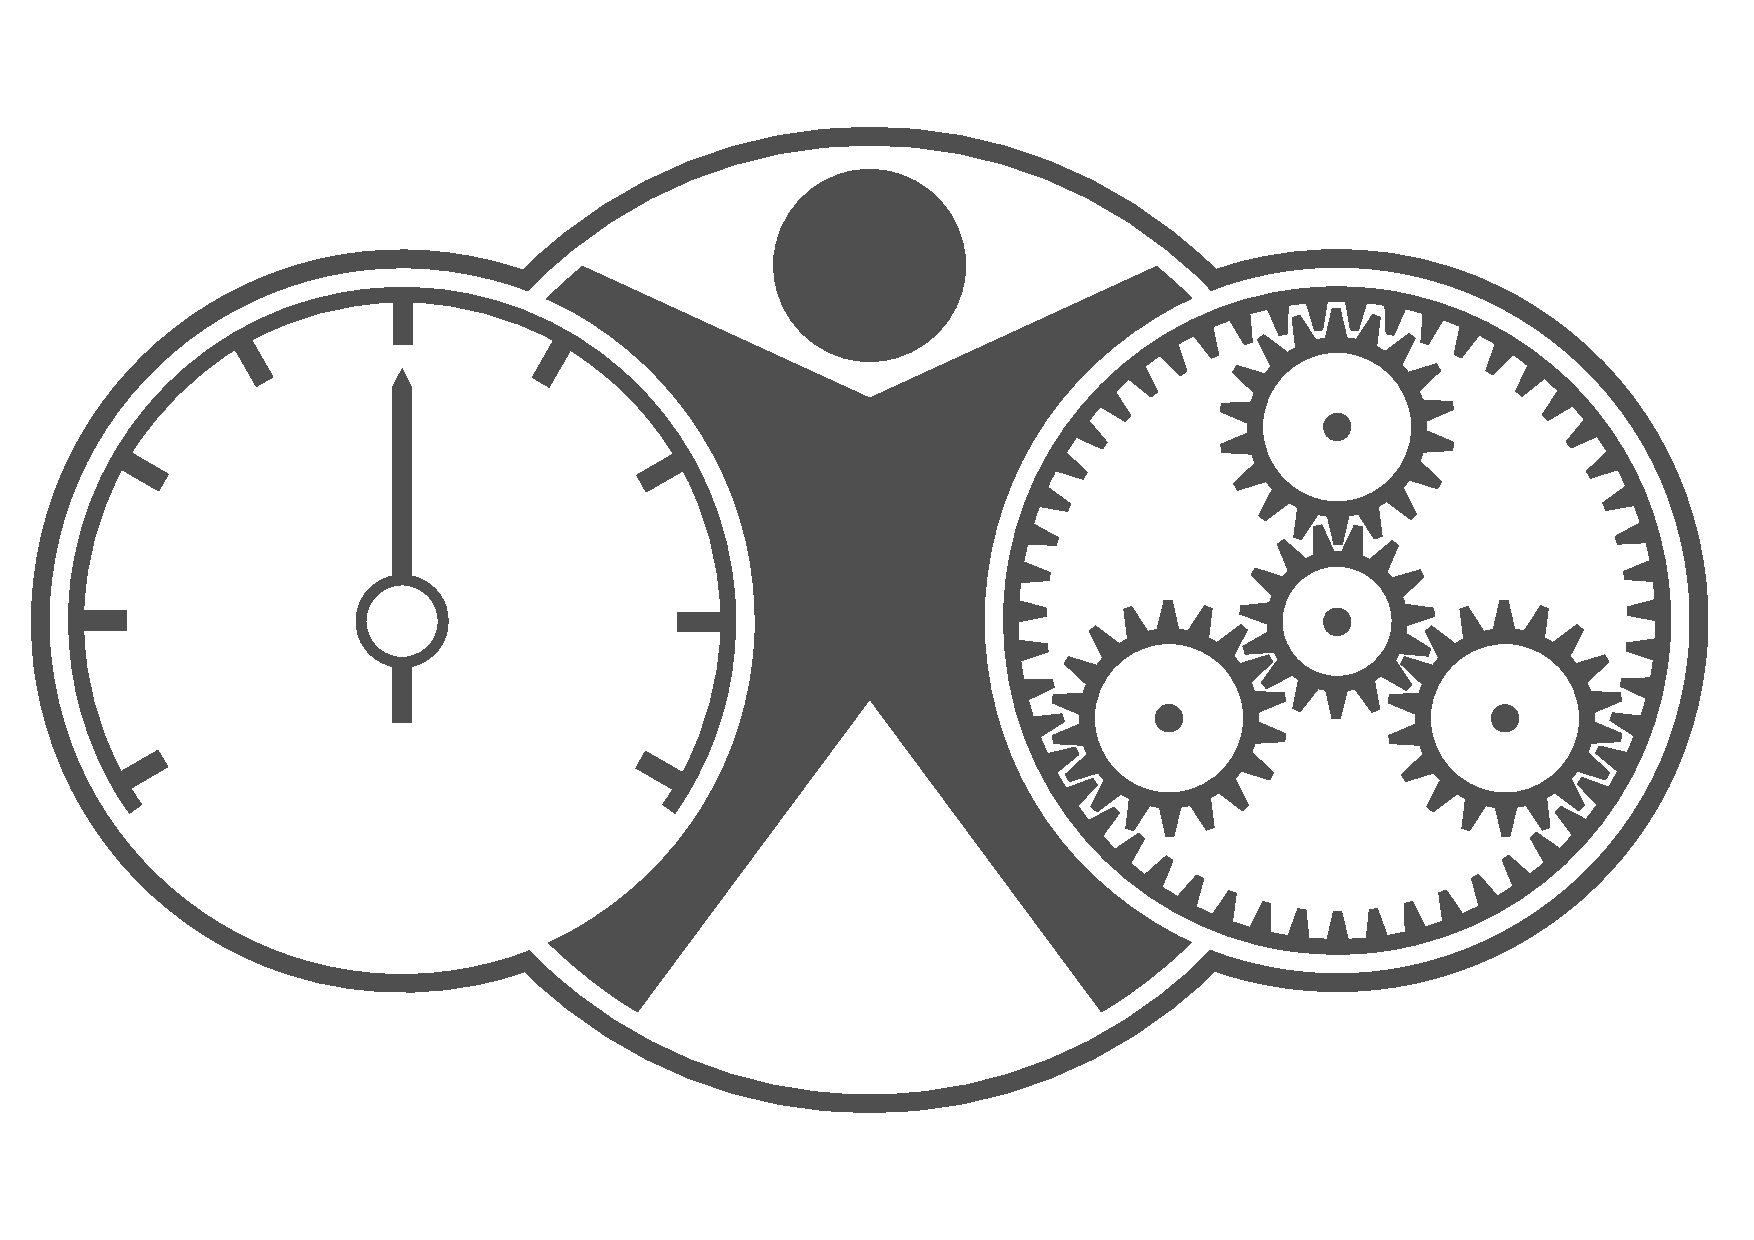
\includegraphics[width=2.5cm]{img/lfe.pdf}
			\end{minipage}
   
%   } 

   \hspace{7cm}
   
   %\put(0,0){
			\begin{minipage}[ht]{0.3\textwidth}
			\centering
			
\includegraphics[width=2.3cm]{img/tum.png}
			\end{minipage}
	}   
\end{picture} \\


\ \\
Technische Universit�t M�nchen\\
Lehrstuhl f�r Ergonomie 


\vspace{5cm}

{\large\bf \myarbeit}\\

\vspace{1cm}

{\Large\bf \mythema}\\

{\large\bf \mythemaeng}


\vspace{3cm}


{\large\bf \myname}\\


 %Titelseite, wird automatisch erstellt

\renewcommand{\thepage}{\roman{page}} %R�mische Zahlen von Hauptteil

\clearpage

\begin{picture}(0,0) 
   \put(-8,0){
   
			\begin{minipage}[ht]{0.3\textwidth}
			\centering
			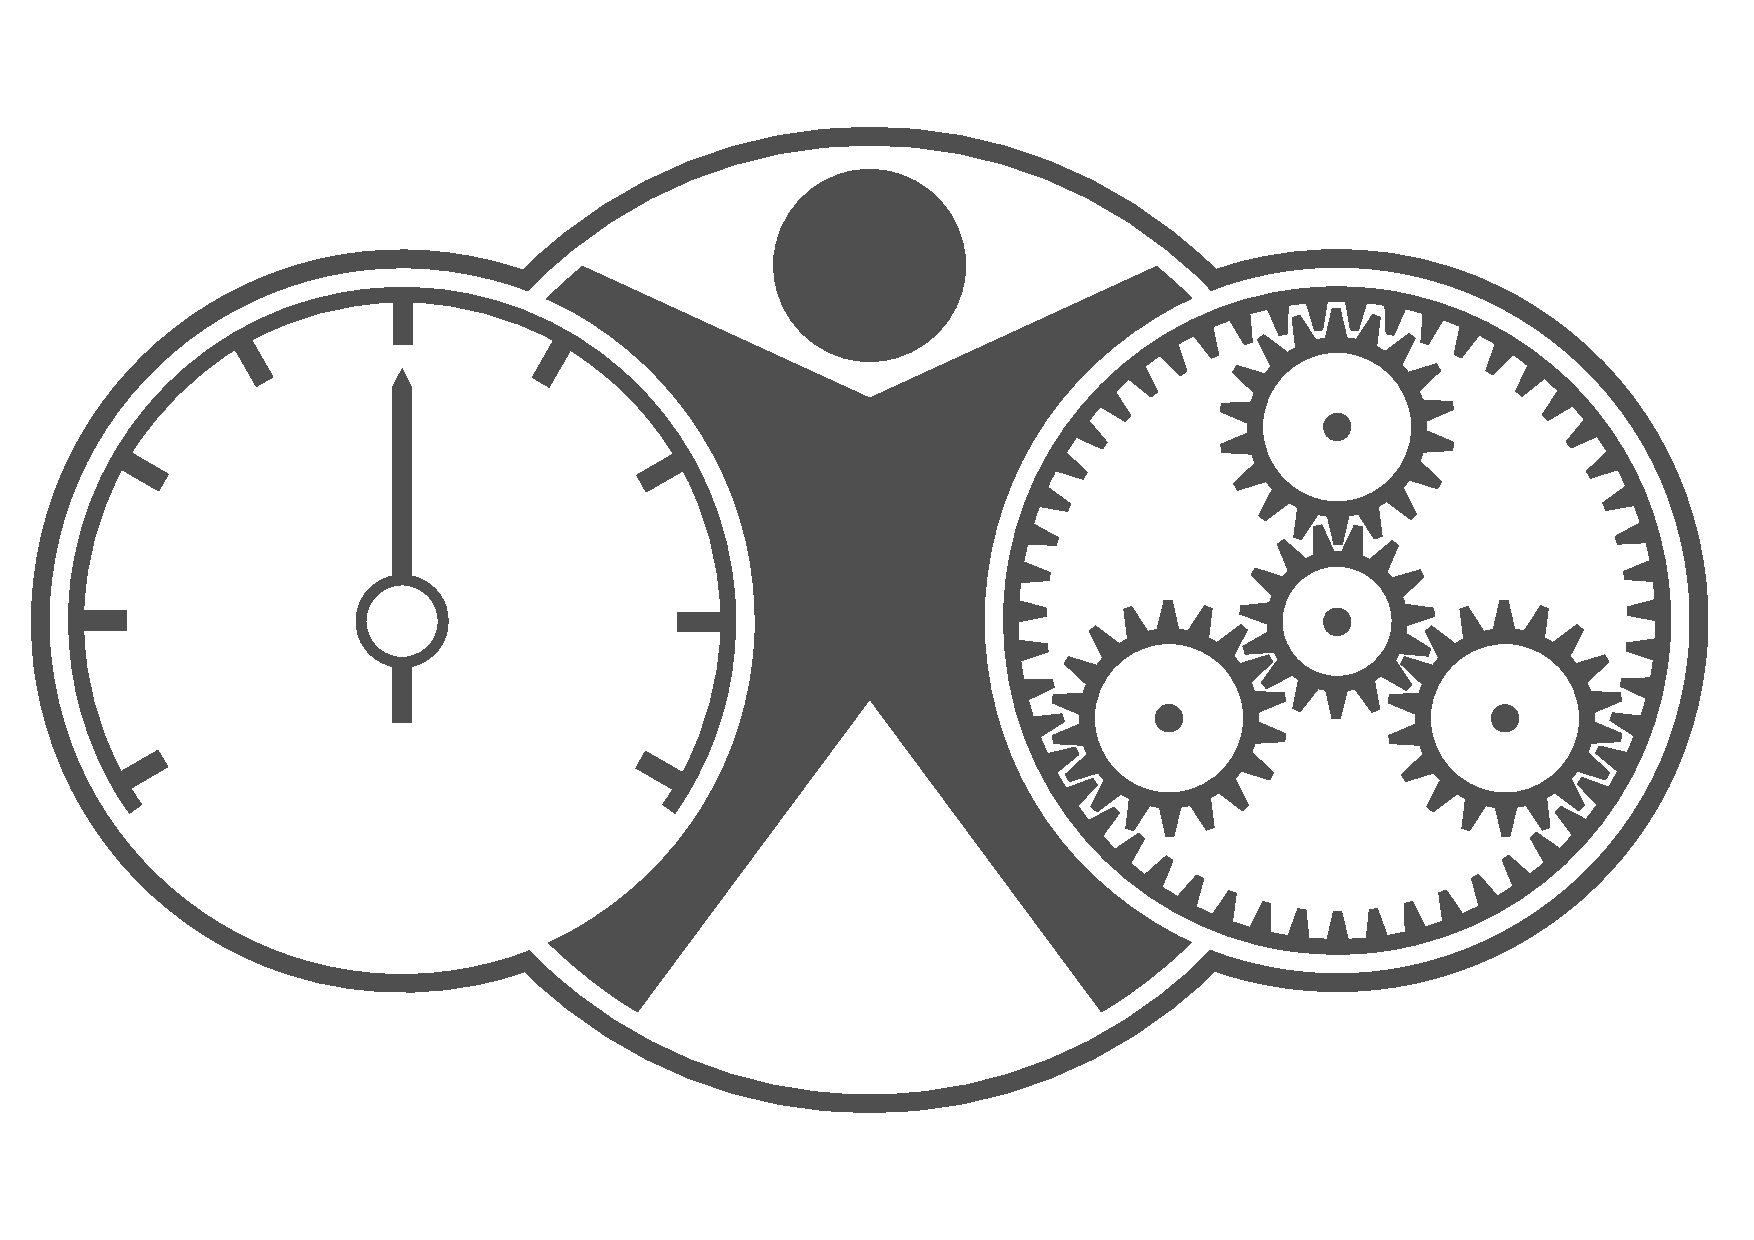
\includegraphics[width=2.5cm]{img/lfe.pdf}
			\end{minipage}
   
%   } 

   \hspace{7cm}
   
   %\put(0,0){
			\begin{minipage}[ht]{0.3\textwidth}
			\centering
			
\includegraphics[width=2.3cm]{img/tum.png}
			\end{minipage}
	}   
\end{picture} \\


\ \\
Technische Universit�t M�nchen\\
Lehrstuhl f�r Ergonomie 

\vspace{3cm}


{\Large\bf \mythema}\\

{\large\bf \mythemaeng}\\

\vspace{1cm}

{\large \myarbeit}\\

\vspace{1cm}


\begin{table}[!hbt]
\large
		\begin{tabular}{ll}
      \vspace{0.5cm}
				Verfasser: & \myname\\
      \vspace{0.5cm}
				Module: & \mymodul\\
      \vspace{0cm}
				Betreuer:	&Univ.-Prof. Dr. phil. Klaus Bengler\\
			\vspace{0cm}
									&Dipl.-Ing. N. N.\\
			\vspace{0.5cm}
									&Dipl.-Inf. N. N.\\						
      \vspace{0.5cm}
				Ausgabe am:&01.01.2012\\
      \vspace{0.5cm}
				Abgabe am:&30.06.2012\\    		
		\end{tabular}
    \vspace{1ex}
\end{table}

 %---------- Bitte anpassen! ----------

\clearpage

\noindent{\Large\bf Eidesstattliche Erkl�rung }\\
\\
Hiermit versichere ich diese Studienarbeit ohne fremde Hilfe selbst�ndig verfasst und nur die angegebenen Quellen und Hilfsmittel verwendet zu haben. W�rtlich oder dem Sinn nach aus anderen Werken entnommene Stellen sind unter Angabe der Quellen kenntlich gemacht.\\
\\
Garching, den\vspace{2.5cm}\\\myname\\

\vspace{3cm}

\noindent{\Large\bf Vereinbarung zum Urheberrecht}\\
\\
Hiermit gestatte ich dem Lehrstuhl f�r Ergonomie diese Studienarbeit bzw. Teile davon nach eigenem Ermessen an Dritte weiterzugeben, zu ver�ffentlichen oder anderweitig zu nutzen. Mein pers�nliches Urheberrecht ist �ber diese Regelung hinaus nicht beeintr�chtigt. 

Eventuelle Geheimhaltungsvereinbarungen �ber den Inhalt der Arbeit zwischen mir bzw. dem Lehrstuhl f�r Ergonomie und Dritten bleiben von dieser Vereinbarung unber�hrt.\\
\\
Garching, den\vspace{2cm}\\\myname
 %Erkl�rungen, wird automatisch erstellt




% --------------------------------------------------
% -------------------- ABSTRACT --------------------
% --------------------------------------------------


% \begin{abstract}
% \thispagestyle{plain} %F�gt eine Seitenzahl ein
% \ofoot[\pagemark]{\pagemark} %F�gt eine Seitenzahl ein
% 
% \noindent{\bf Kurzfassung / Abstract}\\
% 
% 
% Ein Abstract ist eine pr�gnante Inhaltsangabe, ein Abriss ohne Interpretation und Wertung einer wissenschaftlichen Arbeit. In DIN 1426 wird das (oder auch der) Abstract als Kurzreferat zur Inhaltsangabe beschrieben.
% 
% Die Definition des American National Standards Institute (ANSI) lautet: "An abstract is defined as an abbreviated accurate representation of the contents of a document." ("Ein Abstract ist definiert als eine gek�rzte pr�zise Darstellung des Inhalts eines Dokuments.")
% 
% 
% \end{abstract}


% --------------------------------------------------
% --------------- INHALTVERZEICHNIS ----------------
% --------------------------------------------------



\tableofcontents %Bindet das Inhaltsverzeichnis ein

\thispagestyle{plain} %F�gt eine Seitenzahl ein
\ofoot[\pagemark]{\pagemark} %F�gt eine Seitenzahl ein

\clearpage

\phantomsection

\clearpage

\setcounter{page}{4} %Seitenz�hler resetten

% --------------------------------------------------
% ------------------- HAUPTTEIL --------------------
% --------------------------------------------------



\newpage{\pagestyle{plain}
\cleardoublepage}
\renewcommand{\thepage}{\arabic{page}}
\setcounter{page}{1}
\pagestyle{scrheadings}
\renewcommand*{\chapterpagestyle}{scrheadings}

%Es bietet sich an, die einzelnen Kapitel in eigene *.tex Dateien auszulagern, um die �bersichtlichkeit zu verbessern. Sollte das nicht gew�nscht sein, k�nnen die Inhalte dieser *.tex Dateien hier eingef�gt und die "\input xxx.tex"' zeilen entfernt werden.
%Die Gliederung/Kapitel ist/sind nat�rlich der Arbeit entsprechend anzupassen

\chapter{Introduction} \label{cha:introduction}

In the development of new interfaces for the vehicles, or simply in the study of 
the influence in driving performance of some factor of interest, an evaluation
has to be performed. There are different ways to measure the driving quality of
a person under the interest conditions. In particular, there are two important
measurements for this task, the Time to Headway (THW) and the standard deviation
of lateral position (SDLP).

To calculate these measurements is necessary to use points of reference. In the
case of the Time to Headway the point of reference are the vehicles driving in
front of the testing car. In the case of the SDLP measurement, the lanes on the
road are used as the reference point to obtain the lateral position.

In a virtual environment is easy to obtain the exact position of the vehicles
and the lanes on the road, but in the real world is not an easy task. In real
world applications, sensors are used to estimate the position of these reference
points. Unfortunately, sensor measurements generally have some error associated
which is directly associated to the price of the sensor. Expensive sensors like
for example laser scanners are very accurate for distance calculation but at the
same time their price is very high. On the other hand, normal color cameras are
getting more popular to be used as sensors in real world reconstruction due to
its low cost and the recent advances in Computer Vision and Image Processing.

In particular, in the recent years a great number of applications using the
Smartphones cameras have been created. For example, augmented reality
applications that superpose a virtual environment by building references with
the real world through the camera.

Here is where the idea of using a similar application for the problem of
evaluating the driving quality shows up. In particular, to create an application
that uses the camera together with Computer Vision technique to calculate the
THW and SDLP measurements in real-time.

This project is precisely this idea taken to practice. The goal of the current
work is to develop an application
for the Android operative system used by Smartphones and mobile devices for
calculating these two measurements. The project was divided in two modules, one
for each measurement. The first one is the Vehicle Detection Module and is the
one responsible for calculate the THW. The second one is called Lane Detection
Module and is the responsible for the detection of the road lanes and the SDLP
calculation.


% 
\chapter{Anmerkungen zum Format} \label{kap:anmerkungen}


Tabelle \ref{tbl:tab1} zeigt, dass Tabellen eine kursive �berschrift tagen.


\begin{table}[h]
	\centering
	\caption{\textit{So sieht eine Tabelle aus (Bild)}}
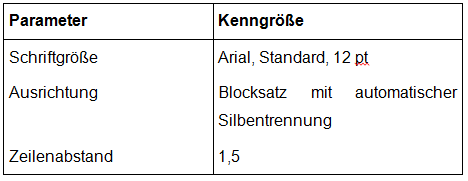
\includegraphics[width=11cm]{img/tabelle.png}
\label{tbl:tab1}
\end{table} 

Tabellen k�nnen entweder als Bild (z.b. aus Excel) eingef�gt werden oder manuell mit LaTeX erstellt werden (siehe \ref{tbl:tab2}):


\begin{table}[h]
	\centering
	\caption{\textit{So sieht eine Tabelle aus (LaTeX)}}	
	\begin{tabular}{|p{3cm}|p{5cm}|}
 			\hline
			\textbf{Parameter} & \textbf{Kenngr��e}\\
			\hline	
				Schriftgr��e & Arial, Standard, 12 pt\\
				Ausrichtung & Blocksatz mit automatischer Silbentrennung\\
				Zeilenabstand & 1,5\\
			\hline
			\end{tabular}
	\label{tbl:tab2}
\end{table} 


Abbildungen tragen eine kursive Bildunterschrift, wie in Abb. \ref{fig:bild1} zu erkennen.

\begin{figure}[ht]
	\centering

\includegraphics[width=8cm]{img/abbildung.png}
\caption{\textit{So sieht eine Abbildung aus}}
\label{fig:bild1}
\end{figure} 

Verweise auf Kapitel, Tabellen oder Abbildungen mit $\backslash ref\{label\}$.



% \chapter{Sumatra PDF Viewer}  \label{kap:sumatra}

Statt den Adobe Reader zu verwenden, bietet sich f�r die Arbeit mit TeXnicCenter der Sumatra PDF-Viewer an. Dieser erm�glicht es, das PDF-Dokument w�hrend der Bearbeitung mit TeXnicCenter ge�ffnet zu lassen. Das PDF-Dokument aktuallisiert sich au�erdem nach der Ausgabe automatisch und die Ansicht bleibt an der entsprechenden Stelle im Dokument.\\

Der Sumatra PDF Viewer ist Freeware und sehr schlank.
Er liegt dieser Vorlage als "SumatraPDF-2.1.1-install.exe" bei, oder steht
auf der Seite des Herstellers zum Download bereit:\\

http://blog.kowalczyk.info/software/sumatrapdf/download-free-pdf-viewer-de.html \\

Nach der Installation muss noch die Einstellung des TeXnixCenter f�r die Verwendung von Sumatra angepasst werden.

Eine Anleitung findet sich in "Sumatra Einrichtung.pdf" oder hier:\\

http://www.texniccenter.org/resources/tutorials


\chapter{Vehicle Detection Module}  \label{kap:vehicle-detection}

Object detection is an important problem appearing on many science fields and
applications like for example robotics, medical science, surveillance systems, etc. The
goal is to detect or determine the presence of a particular object of interest
given a set of measurements obtained from sensors. In the particular context of
computer vision, cameras are commonly used as the sensors and the images they
produce are the measurements.

In this project one of our interest is precisely to detect objects in images 
obtained form a cellphone camera. Specifically the goal is to detect vehicles and 
be able to get the distance between them and the camera. In this
chapter the theory and the method that was considered to
tackle this problem is presented.

\section{Object detection and image classification} % (fold)
\label{sec:objectdetec}

In this section is going to be explained the theoretical framework involved
in the process of detecting objects in camera images. As the reader may know,
there does not exist a definite solution to this problem due to its inherent
complexity. Through the years many interesting strategies have being proposed to
tackle this problem and some of them have shown very good results.

In particular, the work of \cite{viola-jones} in face detection is very
important inside the computer vision community and is the origin for many state
of the art methods used nowadays for object detection. The idea of this work was
to use Machine Learning techniques to learn the intrinsic properties of the
underlying texture produced by a particular object in a image. These underlying
properties are extracted using \textit{features} which consequently are
used to \textit{classify} a texture.

For this project, our goal is to find the set of features that describe the
texture produced by a vehicle and classify those regions in the image with these
features as the detected vehicles. The first step is to define the type of features
that are going to be extracted from the images, then describe the
machine learning algorithm used to extract the particular subset of feature that
describe a vehicle and finally some words about the data used in the learning
process.

\subsection{Feature calculation} % (fold)
\label{sub:Features}

In computer vision and image processing, the term \textit{feature} is commonly 
used for structures or pieces of information that are relevant when analysing an
image. There are uncountable examples of features that can be extracted from an 
image like points, edges, areas, averages of intensities, etc. A particular set
of features and the way to extract them from the image may vary depending on the
application.

For object detection, the set of features used should be robust to capture and
describe the particular textural properties produced by the object of interest.
A particular example in the work of \cite{viola-jones} for face detection, they 
use the well known \textit{Haar-like} features. These features basically compare
the intensity of different regions in the image. This is a particular good
choice of features because when thinking about faces in general, regions like 
the forehead and nose tend to be more illuminated than the region of the eyes 
or beneath the nose. 

Altough Haar-like features have been used in vehicle detection applications, we
opt by using other type of features called \textit{Local Binary Patterns}. First
propposed by \cite{ojala}, the LBP features are one of the best texture
descriptors. They have proven to be highly discriminative and their key advantages,
namely, their invariance to monotonic gray-level changes and computational
efficiency, make them perfect for real-time image processing applications.

The basic idea of LBP features is to summarize the local structure in an image
by comparing each pixel with its neighborhood. For instance, each pixel in the 
neighborhood is compared in terms of intensity to the central pixel. If the
intensity value is higher than the central pixel, it is marked as 1 and 0
otherwise. At the end of the process the neighborhood of each pixel will have a
binary pattern. This basic process is ilustrated in the figure~\ref{fig:lbp}. 

\begin{figure}
\begin{center}
    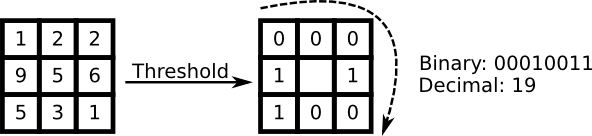
\includegraphics[scale=1.0]{img/lbp.png}
\end{center}
\caption{Ilustrated example in the calculation of the Local Binary Pattern for a
pixel with neighborbood of size 8.}
\label{fig:lbp}
\end{figure}

More formally the LBP extraction can be defined as an operator in the following
manner

\begin{equation*}
    LPB(x_c, y_c) = \sum^{P-1}_{p=0}{2^ps(i_p - i_c)}
\end{equation*}

Where $(x_c, y_c)$ are the coordinates if the central pixel. The intensity of
the central pixel $i_c$ is thresholded with the intensity $i_p$ of the neighbor
$p$ through the function $s$ defined as 

\begin{equation*}
    s(x) =
    \begin{cases}
        1        & \text{if } x \geq 0 \\
        0        & \text{otherwise}
    \end{cases}
\end{equation*}

Finally the binary pattern is stored in form of decimal suming the corresponding
powers of 2.

Nevertheless this simple operator is to illustrate the main idea
of LBP because its fixed neighborhood fails to capture details at different
scales. For this reason, there have been many attemps to extend the LBP operator
to overcome this problem. One particular example is in the work of
\cite{ahonen} called \textit{Extended LBP} or \textit{Circular LBP}. This
extension for the LBP considers a arbitrary number of neighbors at a radial
distance from the central pixel. Formally the coordinates for the neighbor pixel
$p$ are expressed as

\begin{align*}
    x_c &= x_c + R \cos(\frac{2\pi p}{p}) \\
    y_c &= y_c - R \sin(\frac{2\pi p}{p}) \\
\end{align*}

Where $R$ is the distance to the central pixel. When these coordinates do not
correspond to image coordinates, the intensity is calculated by a bilinear
interpolation. In the figure~\ref{fig:lbp-invariant} is reflected the property
of this operator of being invariant to monotonic changes in the intensity.

To incorporate the spatial information, \cite{ahonen} proposed to divide the
image in uniform regions and extract from each one a histogram of the binary
patterns. The histograms from each region are concatenated to form the final
feature vector of the image. This feature vector is also known as
\textit{Local Binary Patterns Histograms}.

\begin{figure}
\begin{center}
    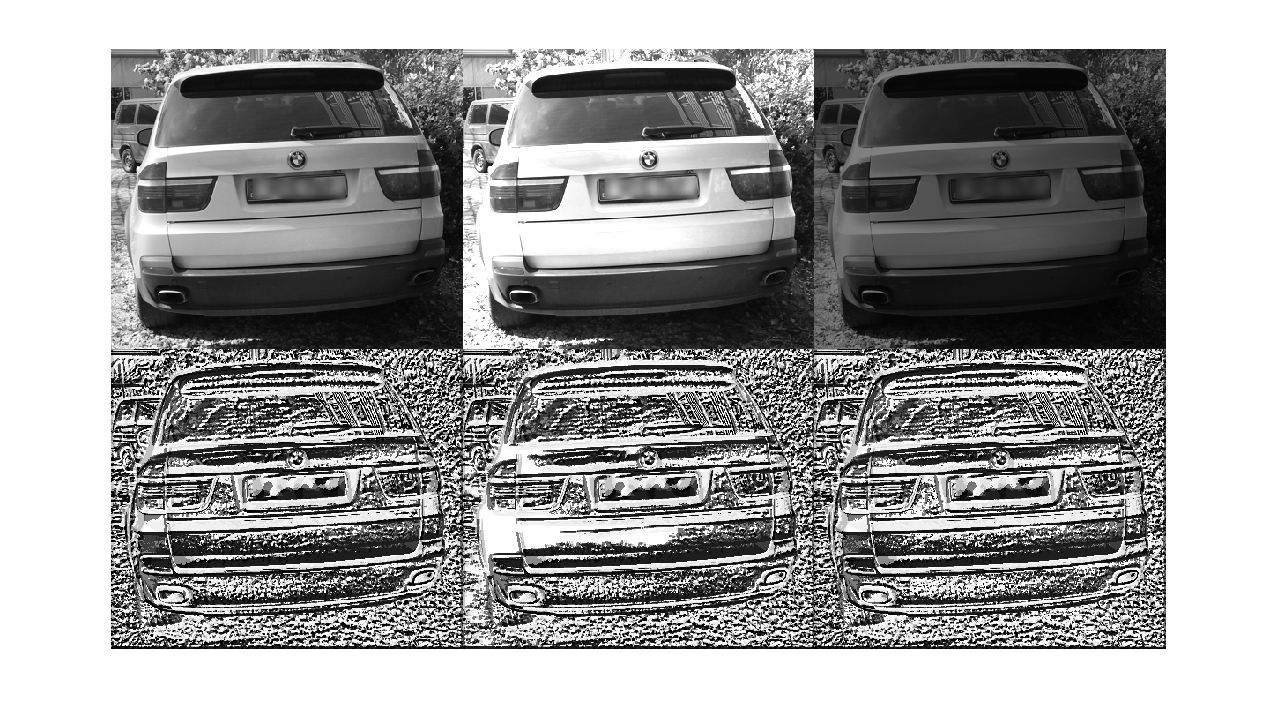
\includegraphics[scale=0.3]{img/invariance.png}
\end{center}
\caption{Local Binary Patterns invariance to constant intensity changes}
\label{fig:lbp-invariant}
\end{figure}

% subsection Features (end)


\subsection{Feature learning} % (fold)
\label{sub:feature-learning}

In the previous section was explained the type of features that are extracted
from the images. The next step is to learn which group of them better describe
the object of interest. In order to do this, a Machine Learning
algorithm is used. In particular, in the work of \cite{viola-jones} they used the
\textit{Adaboost} algorithm. 

Short for ``Adaptive Boosting'', this algorithm was first proposed by
\cite{freund}. In this particular type of boosting, \textit{weak} classifiers
are collected iteratively in a way they adapt to the errors of previously
selected classifiers. The final \textit{strong} classifier is build based on the
votes of each weak classifiers. 

Weak classifier is a name commonly used in Machine Learning to denote hypothesis 
functions that perform slightly better than random in the \textit{training data
set}. In other words, given a set of mixed pictures of vehicles and non-vehicles, a
weak classifier should be able to separate them in a way that the number of
correctly classified pictures is slightly larger than the incorrect ones. The
classification is perform not directly on the images but in the feature vector
extracted from them.

In the training phase every training example, meaning every picture of a
vehicle or non-vehicle, has a weight associated to it. On each iteration, the
weights of the training examples wrongly classified will increase and the
weights of the correctly classified will decrease. This makes that in each
iteration the selected classifier will be prioritize the correct classification
of those training examples with higher weights. In the figure~\ref{fig:adaboost}
you can find an illustration of this idea.

\begin{figure}
\begin{center}
    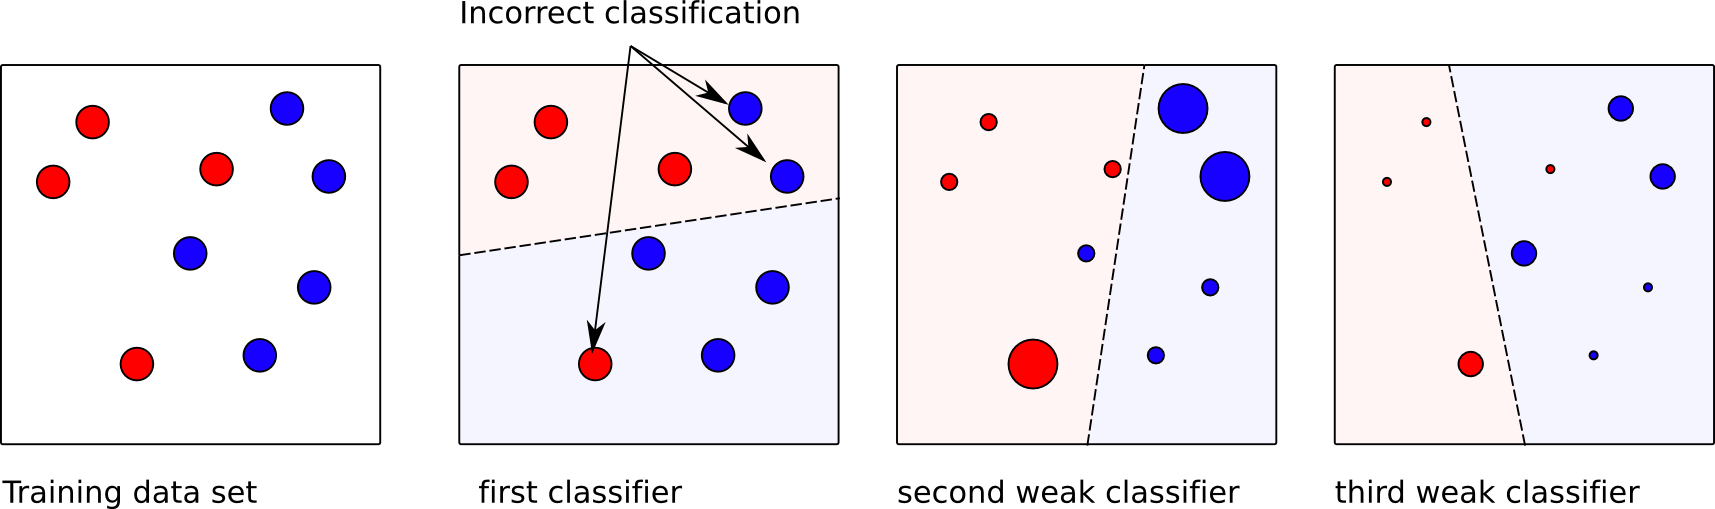
\includegraphics[scale=0.6]{img/adaboost.png}
\end{center}
\caption{Illustration of the AdaBoost algorithm learning. The weak classifiers
are represented by lines separating the training examples in a hypothetical 2D
feature space. The color represents the class of the object and the size of the
points represents the importance weight.}
\label{fig:adaboost}
\end{figure}

Formally the algorithm is described in the table~\ref{alg:Adaboost}. Note how
the final strong classifier is just a weighted sum of the votes of each weak
classifier. The weighting is given by their performance on the dataset.


\begin{algorithm}
    \caption{Adaboost algorithm}
    \begin{algorithmic}[1]
        % \Require Metric space $(X, d_x)$, some initial point $x_1 \in X$ and the
        % desire sampling radius $r_0$.
        % \Ensure a sampling $X' = \{x_1, \dots, x_N\}$.
        \State Initialize the data weighting coefficients $\{w_n\}$ by setting
        $w_n^{(1)} = \frac{1}{N}$ for $n = 1, \cdots, N$.
        \For {$m = 1, \cdots, N$}
        \State \parbox[t]{\dimexpr\linewidth-\algorithmicindent}
        {Fit a classifier $y_m(x)$ to the remaining data by minimizing
        \begin{equation*}
            J_m = \sum^{N}_{n=1}{w_n^{(m)} I(y_m(x_n) \ne t_n)}
        \end{equation*}
        where $I(y_m(x_n) \ne t_n)$ is the indicator function and equals 1
        when $y_m(x_n) \ne t_n$ and 0 otherwise.}

        \vspace{0.25cm}

        \State \parbox[t]{\dimexpr\linewidth-\algorithmicindent}
        {Evaluate the quantities
        \begin{equation*}
            \epsilon = \frac{\displaystyle\sum^{N}_{n=1}{w_n^{(m)}I(y_m(x_n) \ne
        t_n)}}{\displaystyle\sum^{N}_{n=1}{w_n^{(m)}}}
        \end{equation*}
        and then use these to evaluate
        \begin{equation*}
            \alpha_m = \log\left\{ \frac{1 - \epsilon_m}{\epsilon_m} \right\}
        \end{equation*}
        \strut }

        \State Update the data weighting coefficients
        \begin{equation*}
            w_n^{(m+1)} = w_n^{(m)} \exp\left\{ \alpha_mI(y_m(x_n)) \ne t_n \right\}
        \end{equation*}
        \EndFor
        \State \textbf{end}
        \State Make predictions using the final model, which is given by
        \begin{equation*}
            Y_M(x) = sign\left( \sum^{M}_{m=1}{\alpha_m y_m (x)} \right)
        \end{equation*}
    \end{algorithmic}
    \label{alg:Adaboost}
\end{algorithm}


% subsection feature-learning (end)

\subsection{Dataset construction} % (fold)
\label{sub:data-set}

The final step and maybe the most critical one is the dataset construction. In
Supervise Machine Learning everything is about data. The more data is used,
the more the algorithm can learn and the more it can generalize to all possible scenarios.
Unfortunately, gathering data is usually very expensive process. It is expensive
in terms of quality and quantity.

Moreover, depending on the complexity of the application a minimum amount of data 
is required in oder to obtain meaningful results. The higher the complexity of the 
application, the more data is required. The problem of vehicle detection,
involves a high complexity. First of all because the huge variability on
vehicle's shape and color and secondly because of all the factors that can
influence the image formation, like for example weather conditions.

For this work a set of about 430 pictures of rear view cars was labeled. The
pictures where extracted from the dataset used by \cite{tme} and the Caltech
Computer Vision Dataset of rear cars created by Markus Weber (1999). For the
negative examples, the Caltech background dataset was used, also collected by
Markus Weber. Some of the images used as the training dataset are shown in 
the figure~\ref{fig:dataset}.


\begin{figure}[t]
\begin{subfigure}[b]{0.5\textwidth}
\centering
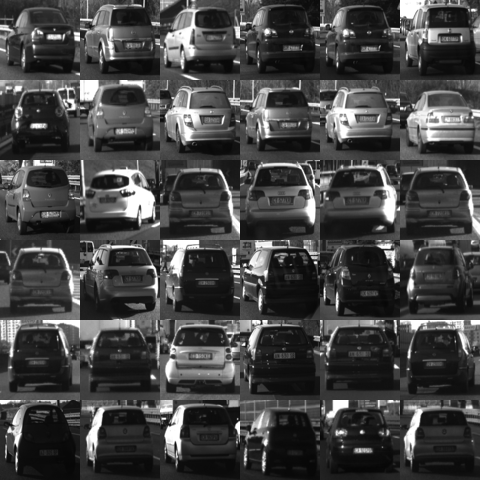
\includegraphics[width=0.85\linewidth]{img/positives.png}
\caption{Positive training examples}
\end{subfigure}
\begin{subfigure}[b]{0.5\textwidth}
\centering
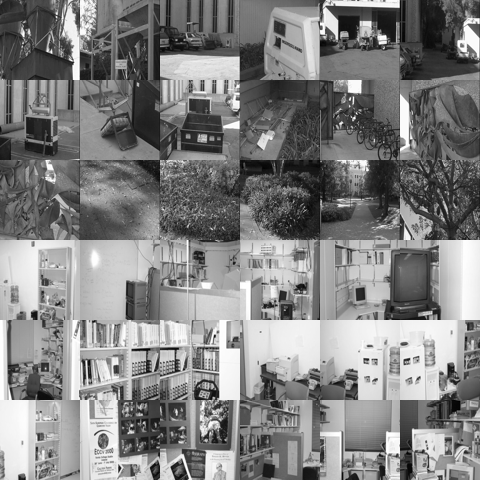
\includegraphics[width=0.85\linewidth]{img/negatives.png}
\caption{Negative training examples}
\end{subfigure}
\caption{Sample of images used as the training set}
\label{fig:dataset}
\end{figure}

% subsection data-set (end)


% section Object detection and image classification (end)

\section{Classification refinement} % (fold)
\label{sec:Classification-refinement}

Due to the great spectrum of different textures appearing in an image, false
classification may occur. This is essentially an inherent problem of the
effort the classifier does to predict unknown data. These mistakes from the
classifier are divided into two types, false positives and false negatives. A
false positives occur when the classifier wrongly label negative examples as 
positive and false negatives is the other way around.

Sometimes it is possible to use some strategies to improve a classification by
removing some of this false classifications. In this particular project, we
suppose a continuous flow of images coming from a camera.
This fact offers an extra dimension which allow us to make assumptions in
order to filter some of the false classifications.

Basically we assume the camera is fixed inside the vehicle, meaning that the images
coming from it should show always the frontal view. This summed to the stream of
images allow us to suppose that a vehicle appearing in one image is going to also 
appear in the next one, in almost the same region inside the image.

With this in mind, it is easy to design a simple strategy to eliminate some
false positives. Supposing a vehicle can not simply disappear from one
frame to the other, a classification window can be constructed over time, where
the position of all the previous classified vehicles is tracked. If a new
classification is not consistent with the previous ones in the window, then it
is simply dropped. 

The final size of the region containing the vehicle is averaged with the
information inside the classification window. This smooths jumps of the region
size returned by the classifier due to the search in different scales.

\begin{figure}    
\begin{minipage}[t]{0.45\textwidth}
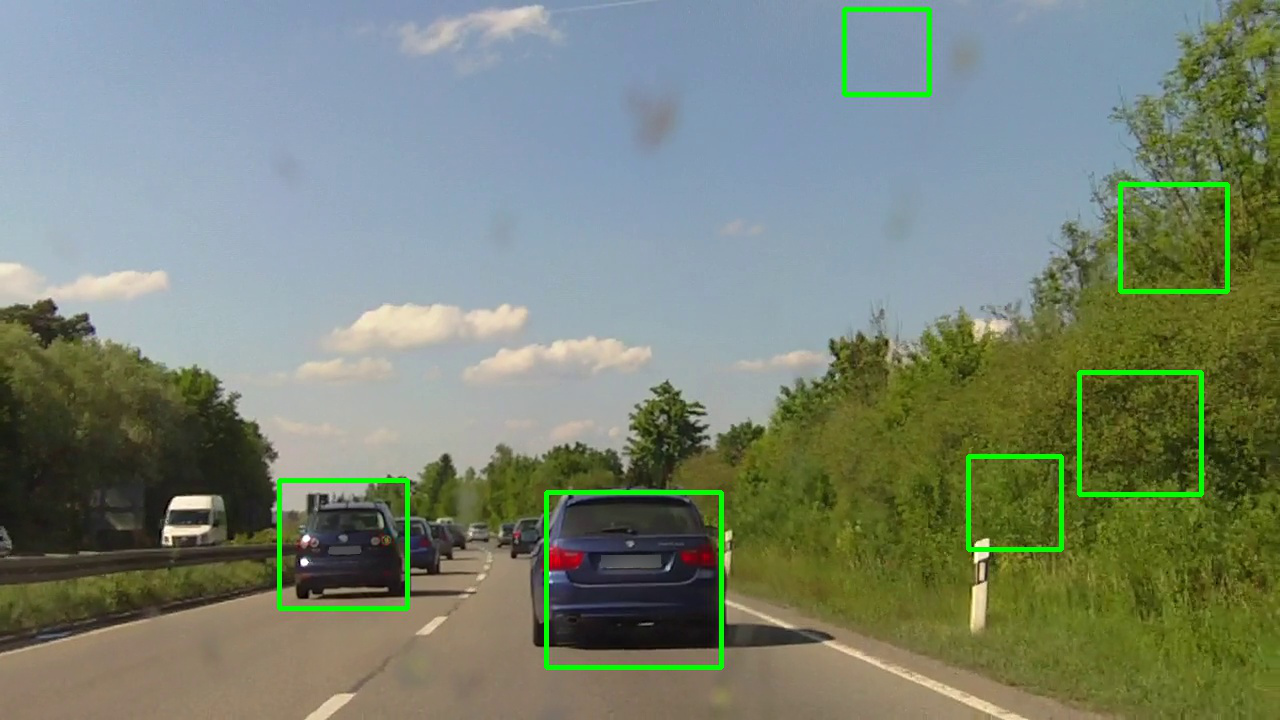
\includegraphics[width=\linewidth]{img/outliers_original.jpg}
\caption{Original classification of the image.}
\end{minipage}
\begin{minipage}[t]{0.45\textwidth}
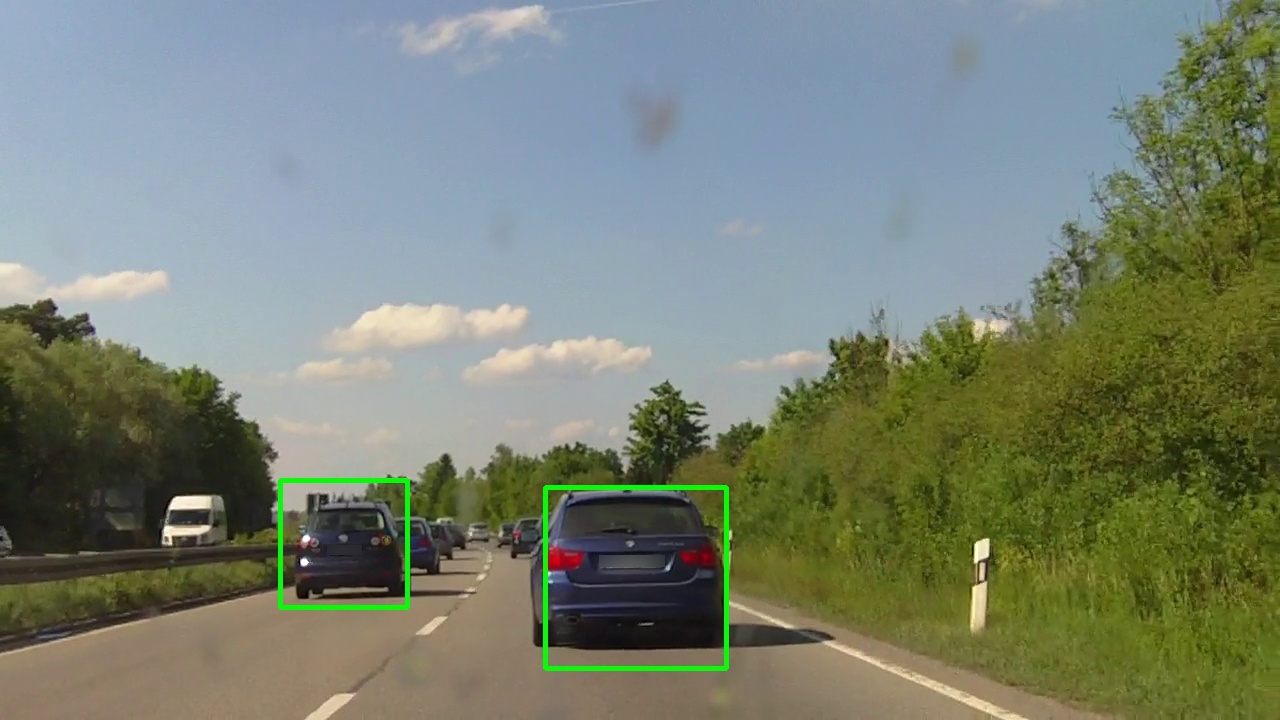
\includegraphics[width=\linewidth]{img/outliers_filtered.jpg}
\caption{False positives filtered with time window strategy}
\end{minipage}
\caption{False positives filtering}
\label{fig:distance-pictures}
\end{figure}

% section Classification refinement (end)

\section{Distance estimation} % (fold)
\label{sec:Distance-estimation}

When projecting the real 3D world through the lenses of a camera into a 2D
image, some information is lost. In particular, the scale and the notion of
distances is lost. It is not possible give any real
measurement of distances in the real world just looking at one image. 
Of course, as humans we can find references in an image from objects we already
know and stablish some scale to compare the rest of the image content. Think for
example of a picture of a small toy car. If the model is realistic 
enough, a human can not differentiate it from a real one, then having an
incorrect estimate of its size.

This problem is discussed in this section and it is required to make some
assumptions to be able to produce a solution. First it is assumed that the
pictures are from real vehicles, this is really
important because our goal is to obtain references of real world distances. The
problem is that generally vehicles have different sizes and shapes. Nevertheless
is not a bad idea to assume an average width for all the vehicles. 

The second problem is that the width in meters of the vehicles is not obtained 
directly from the picture, but a group of pixels containing the image of
the car. To solve this, is necessary to find the relation between the size of
the region containing the vehicle, and the distance to it. For this reason, as a first
approach, we took a number of pictures at different distances of a vehicle. Some of 
these pictures appear in the figure~\ref{fig:distance-pictures}.

\begin{figure}[t]
\begin{subfigure}[b]{0.5\textwidth}
\centering
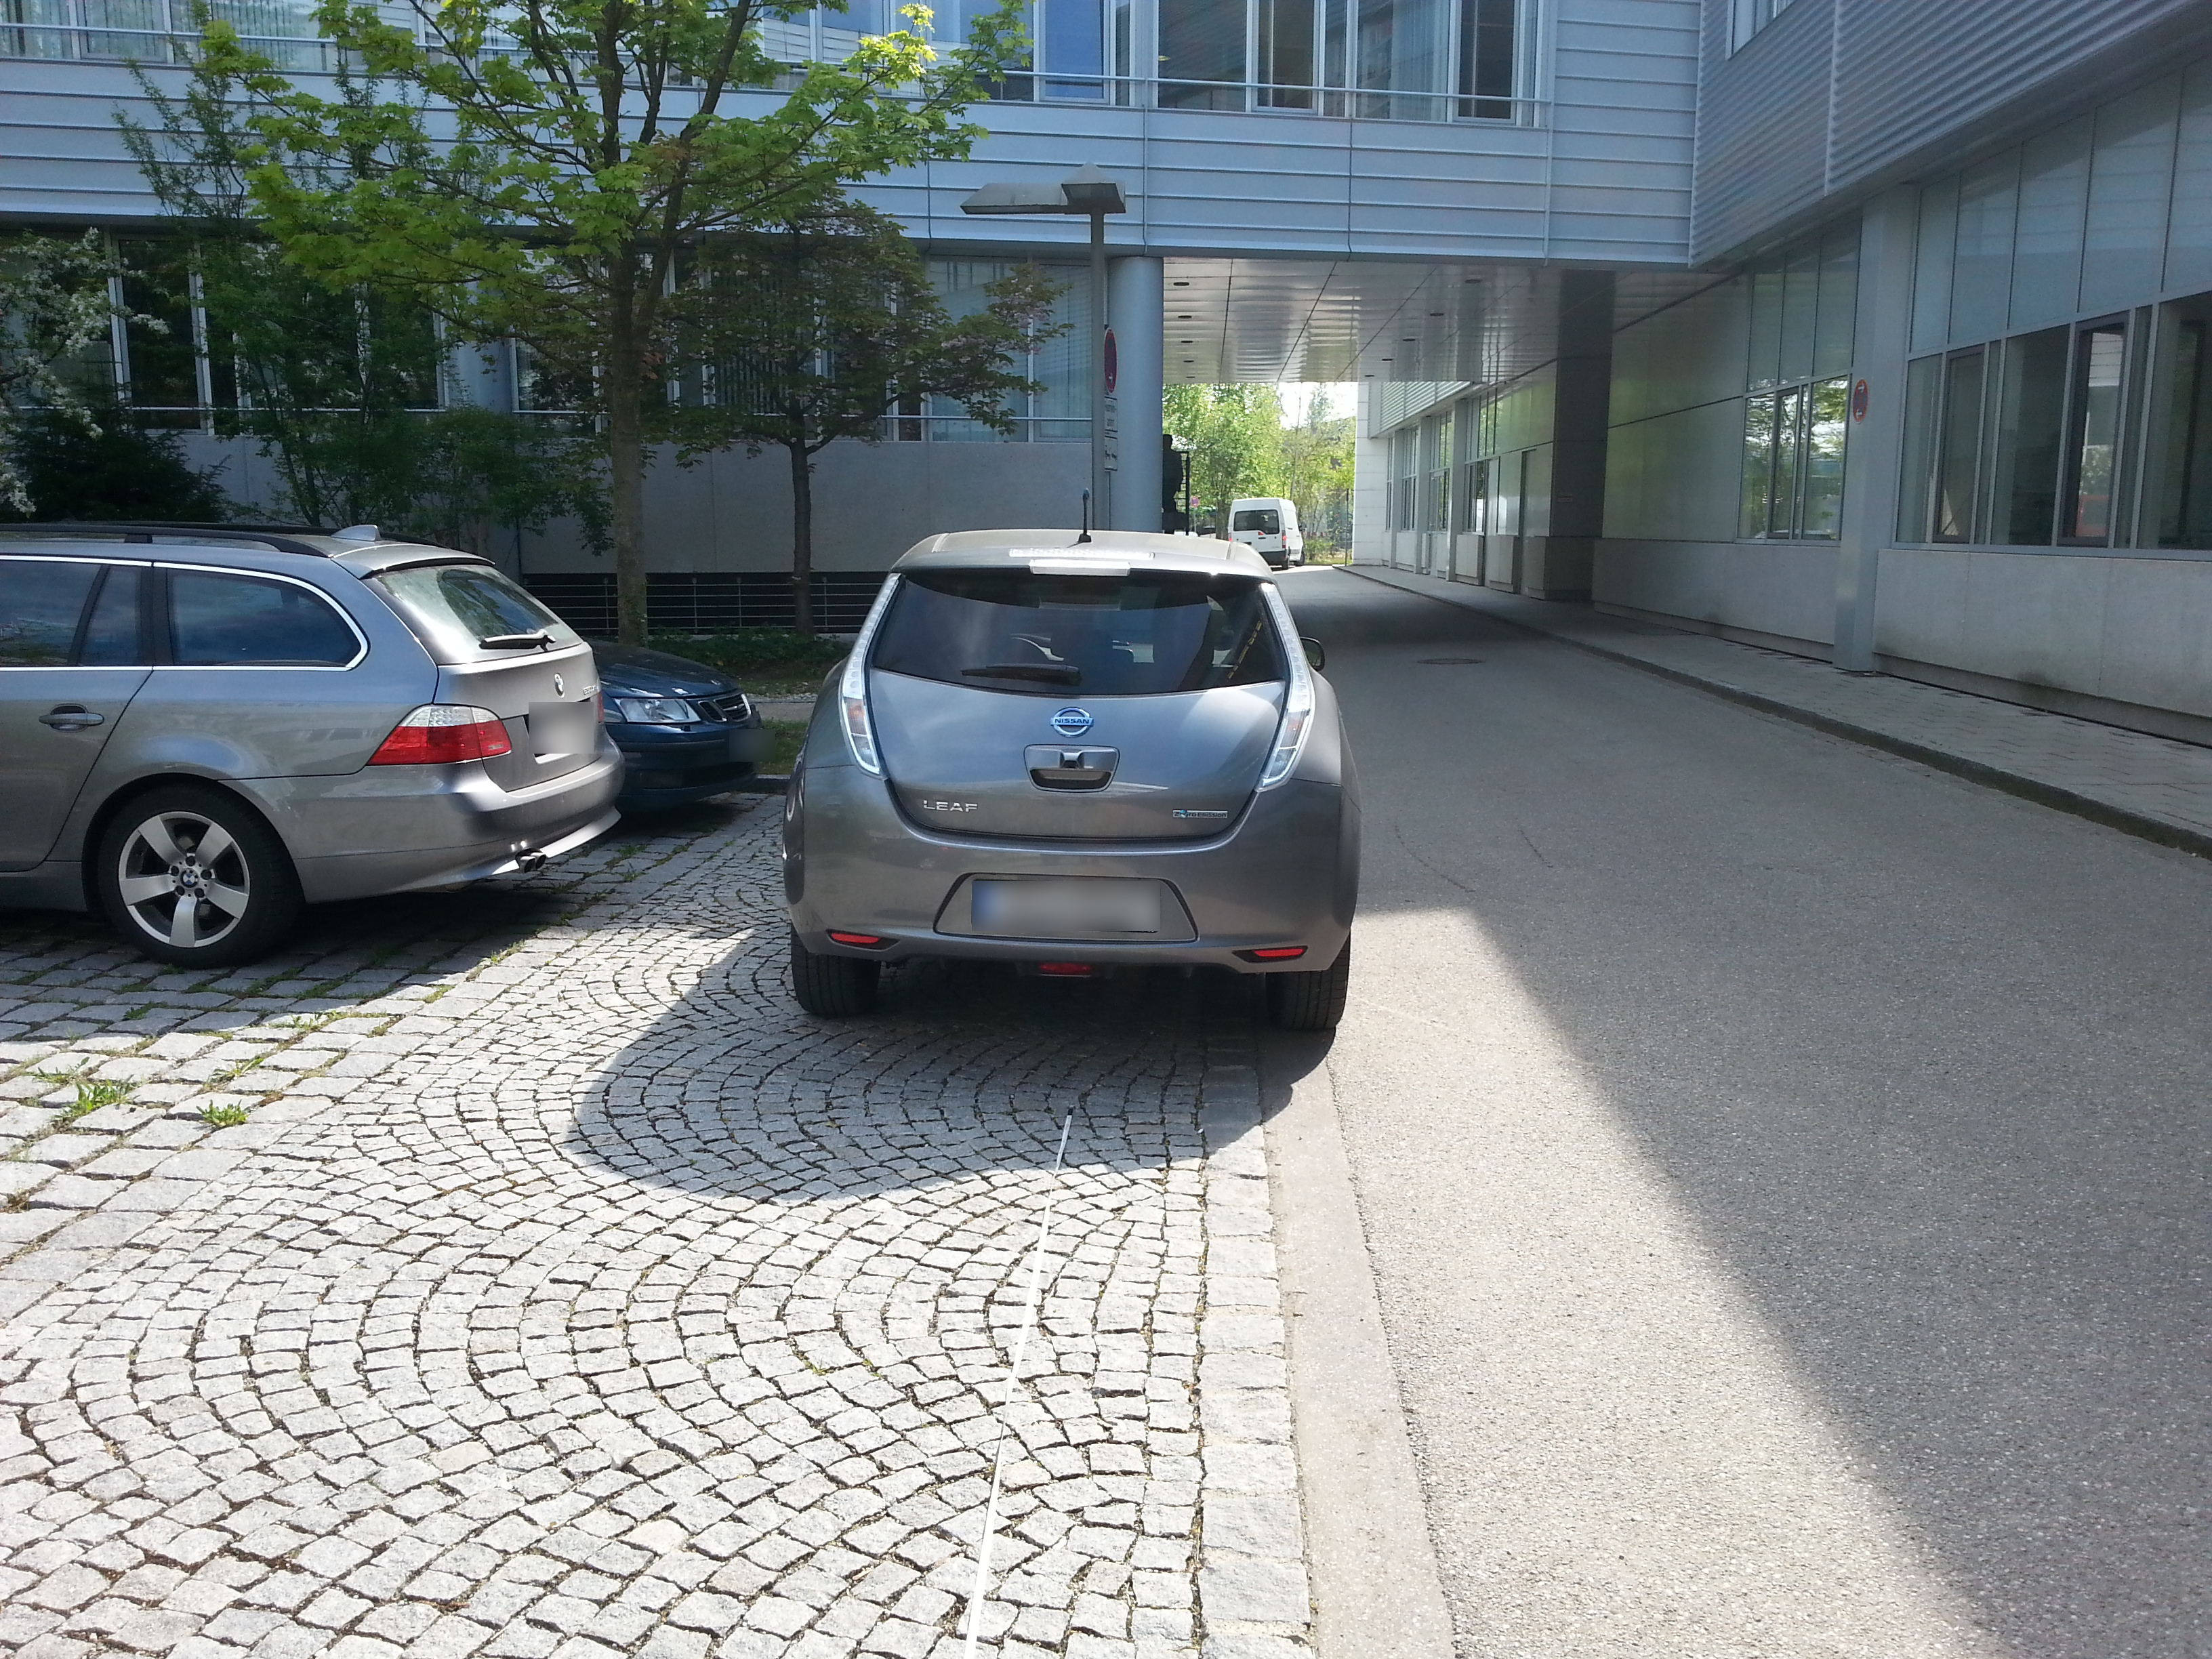
\includegraphics[width=0.75\linewidth]{img/elwoplate5m.jpg}
\caption{Distance of 5 meters to the vehicle}
\end{subfigure}
\begin{subfigure}[b]{0.5\textwidth}
\centering
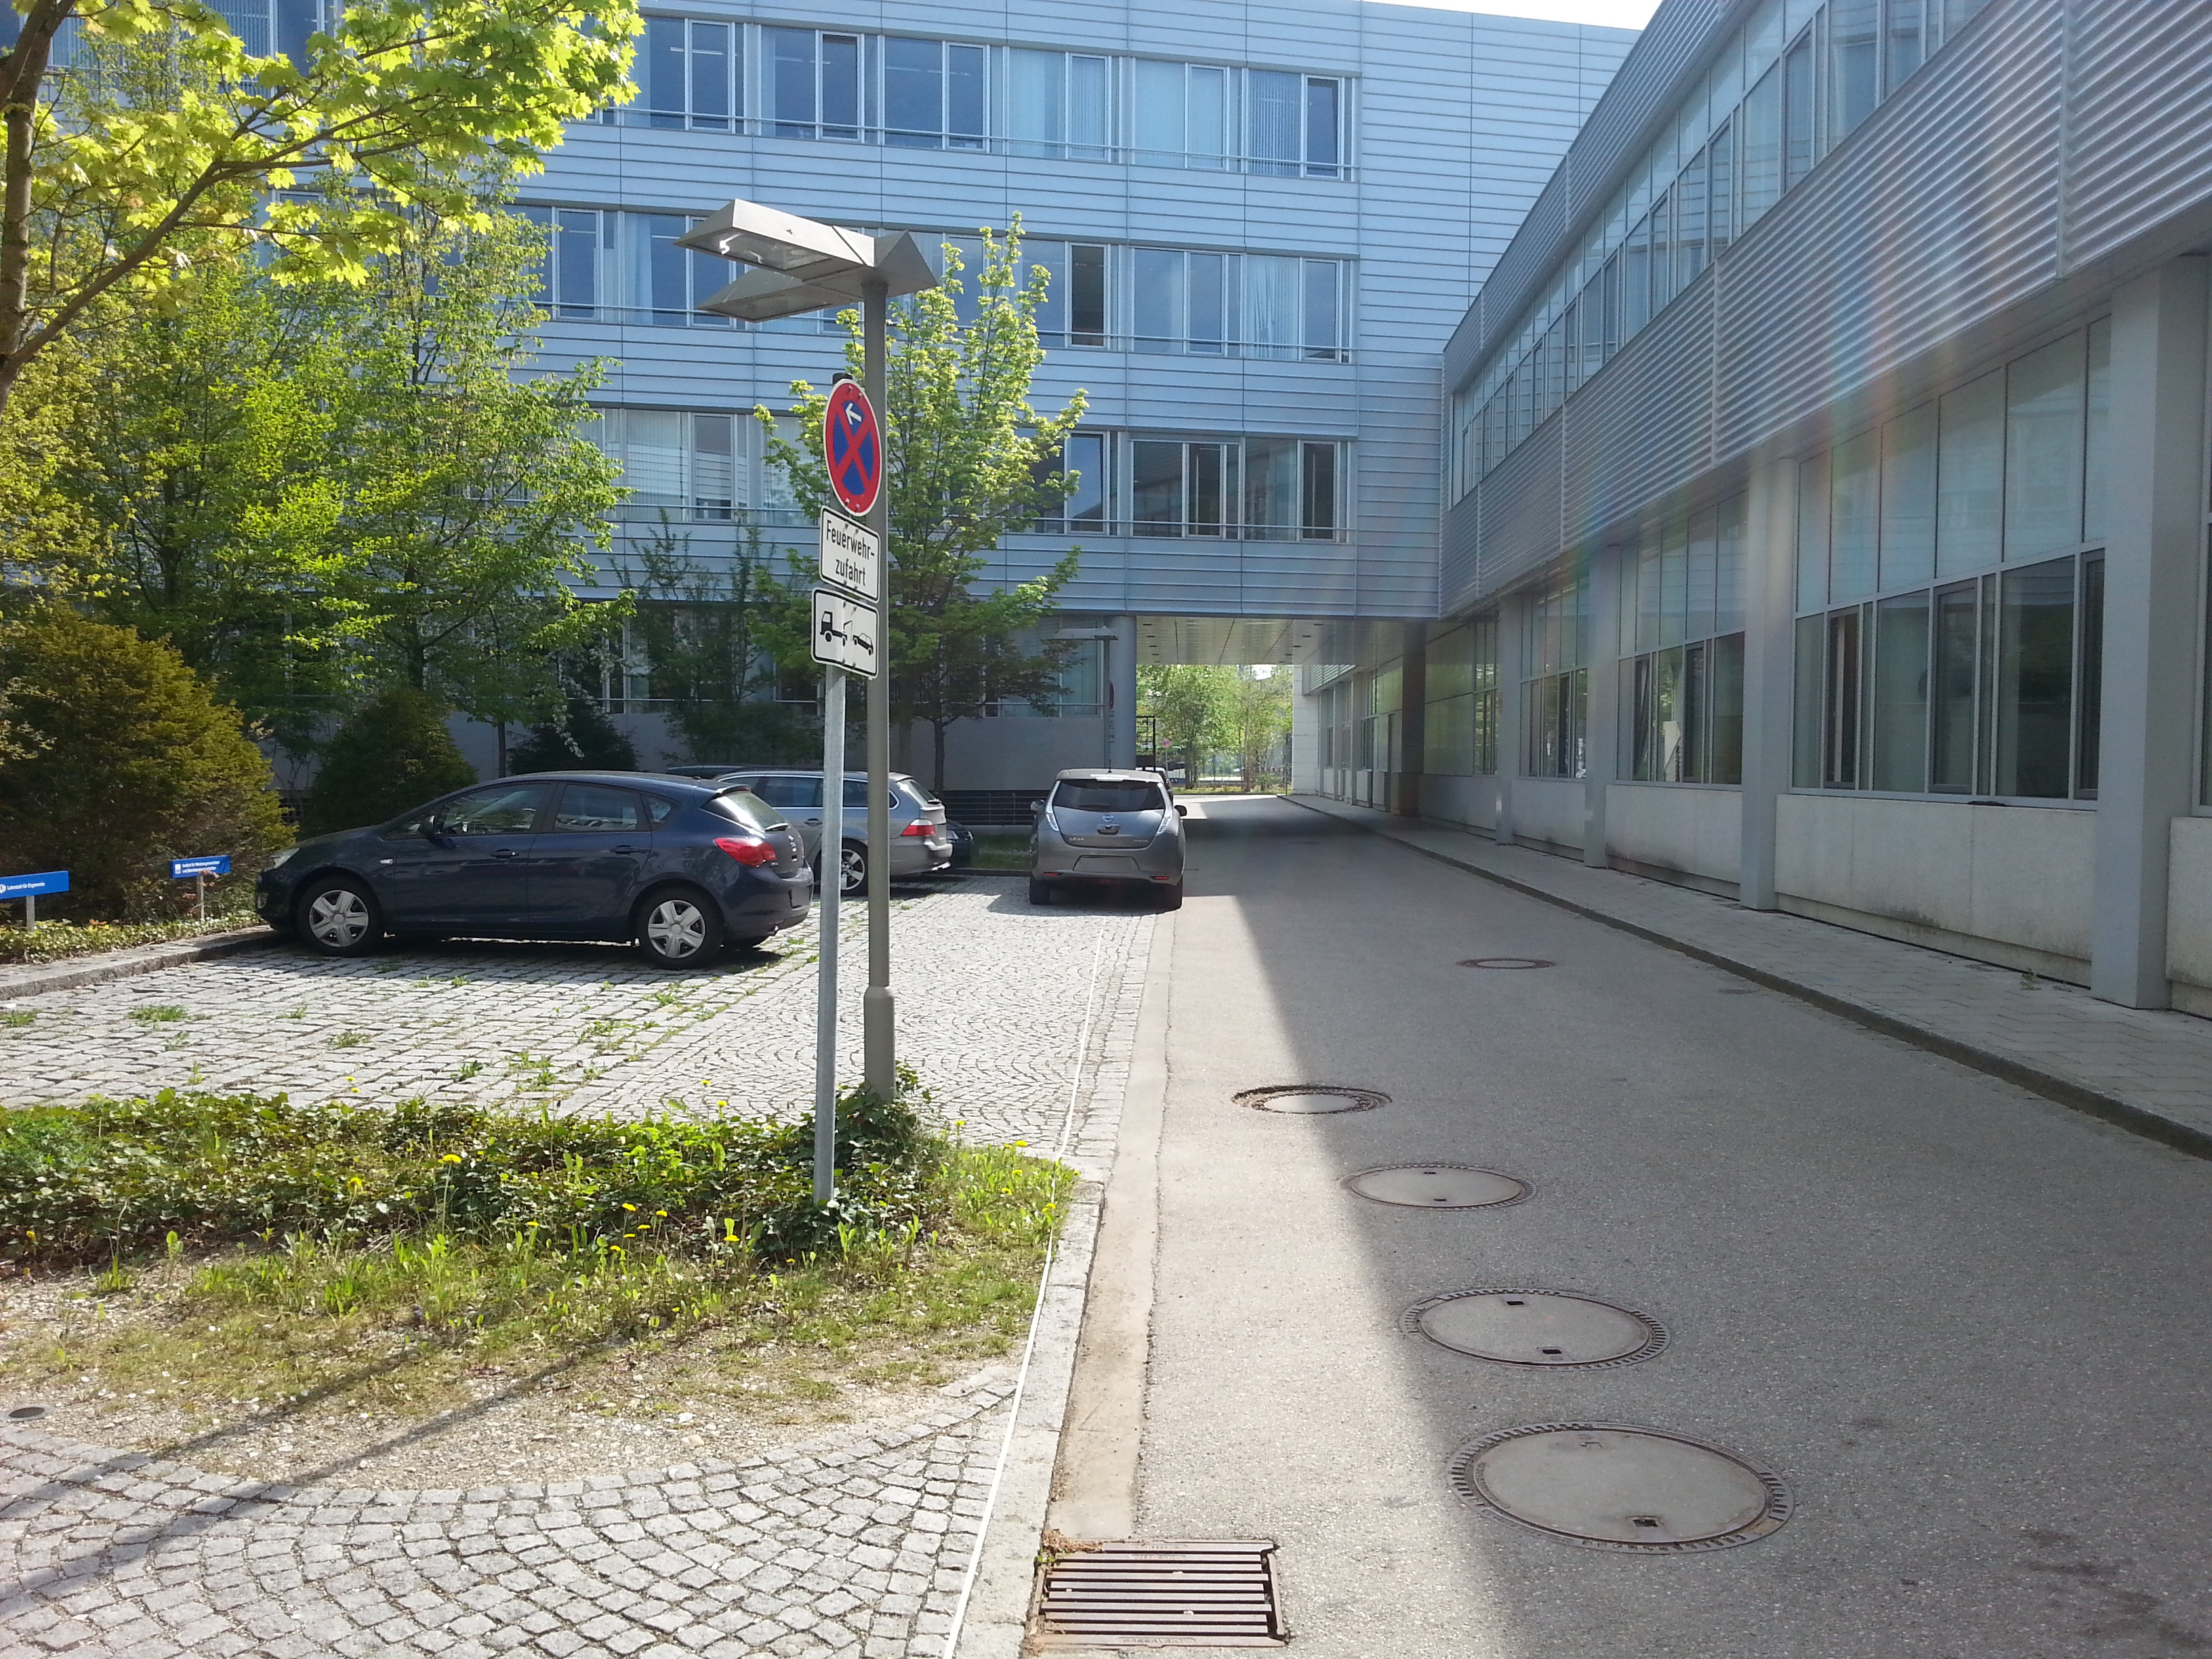
\includegraphics[width=0.75\linewidth]{img/elwoplate20m.jpg}
\caption{Distance of 20 meters to the vehicle}
\end{subfigure}
\begin{subfigure}[b]{0.5\textwidth}
\centering
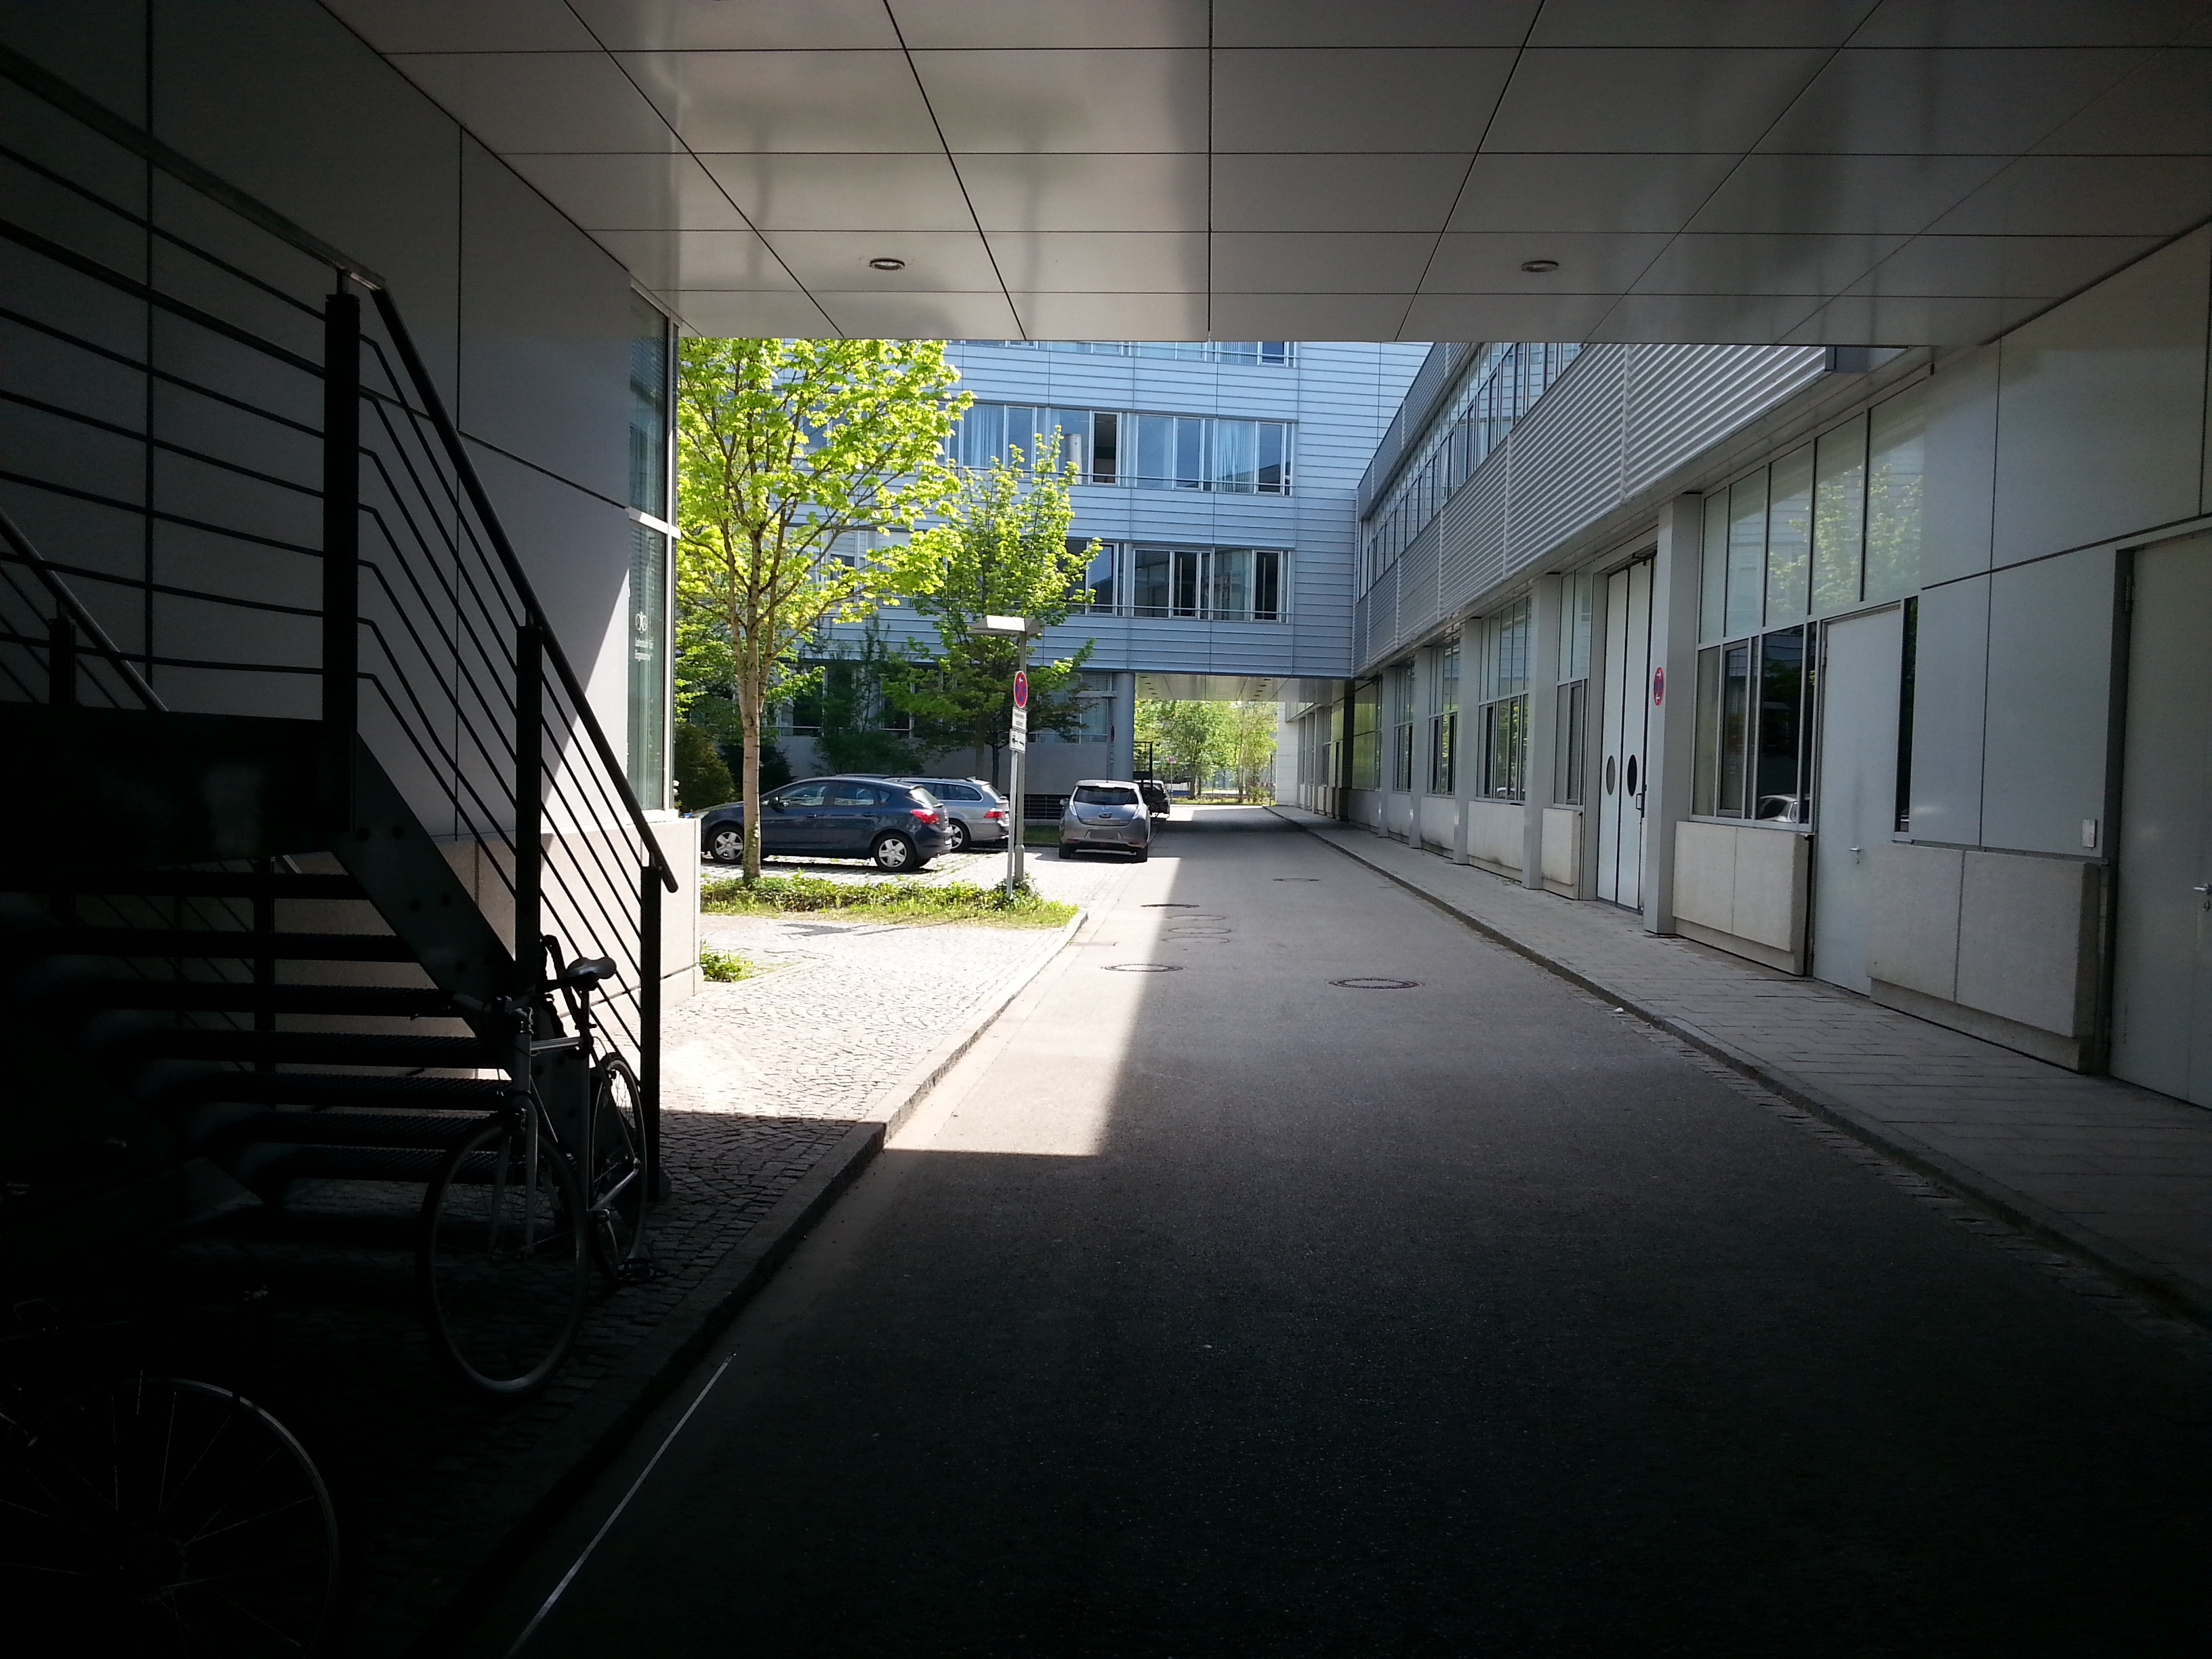
\includegraphics[width=0.75\linewidth]{img/elwoplate35m.jpg}
\caption{Distance of 35 meters to the vehicle}
\end{subfigure}
\begin{subfigure}[b]{0.5\textwidth}
\centering
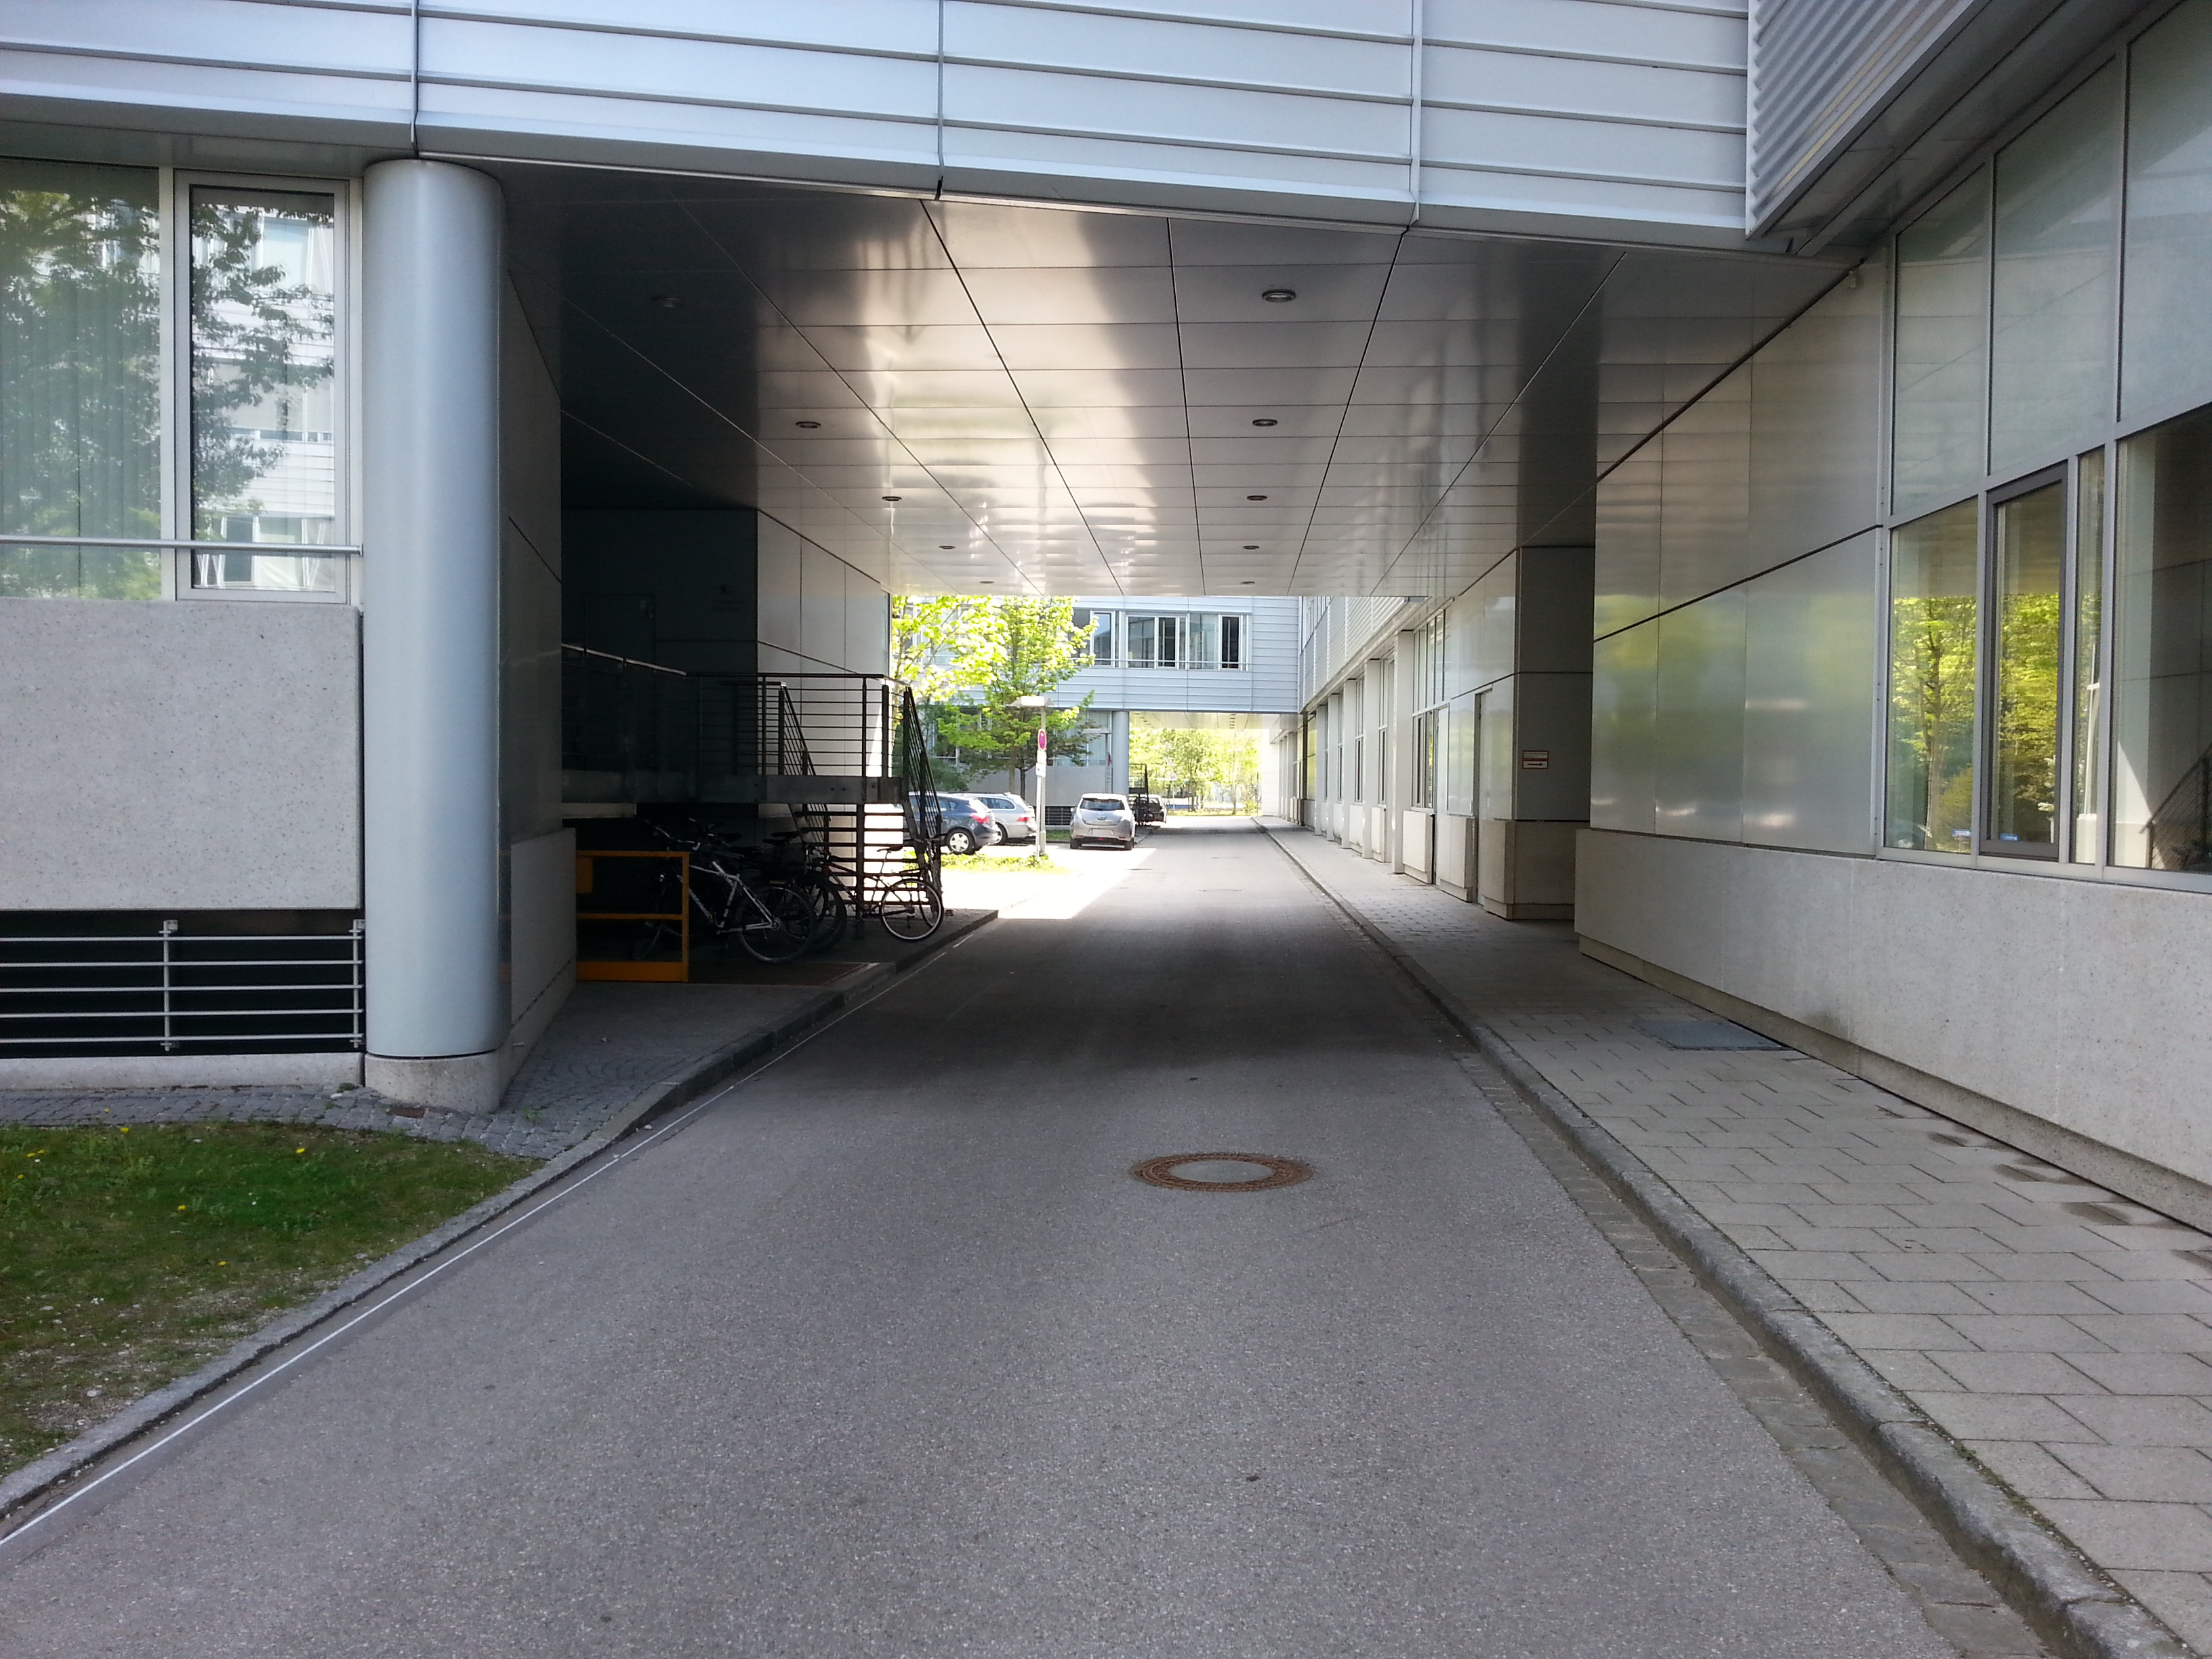
\includegraphics[width=0.75\linewidth]{img/elwoplate50m.jpg}
\caption{Distance of 50 meters to the vehicle}
\end{subfigure}
\caption{Sample of images at different distances from the testing vehicle}
\label{fig:distance-pictures}
\end{figure}

In the figure~\ref{fig:distance-curve-fitting} are displayed as red points, the
measurements obtained from each image. As you can see, this points follows an
exponential function. In order to be able to make a prediction of the distance,
it was decided to fit a exponential model to this data points. The exponential
model selected for this task is given by the next formula

\begin{equation}
    \mathcal{M}(x) = a \cdot \exp(b \cdot x) + c \cdot \exp(d \cdot x)
    \label{eq:distance-curve-model}
\end{equation}

\begin{figure}[h]
\centering
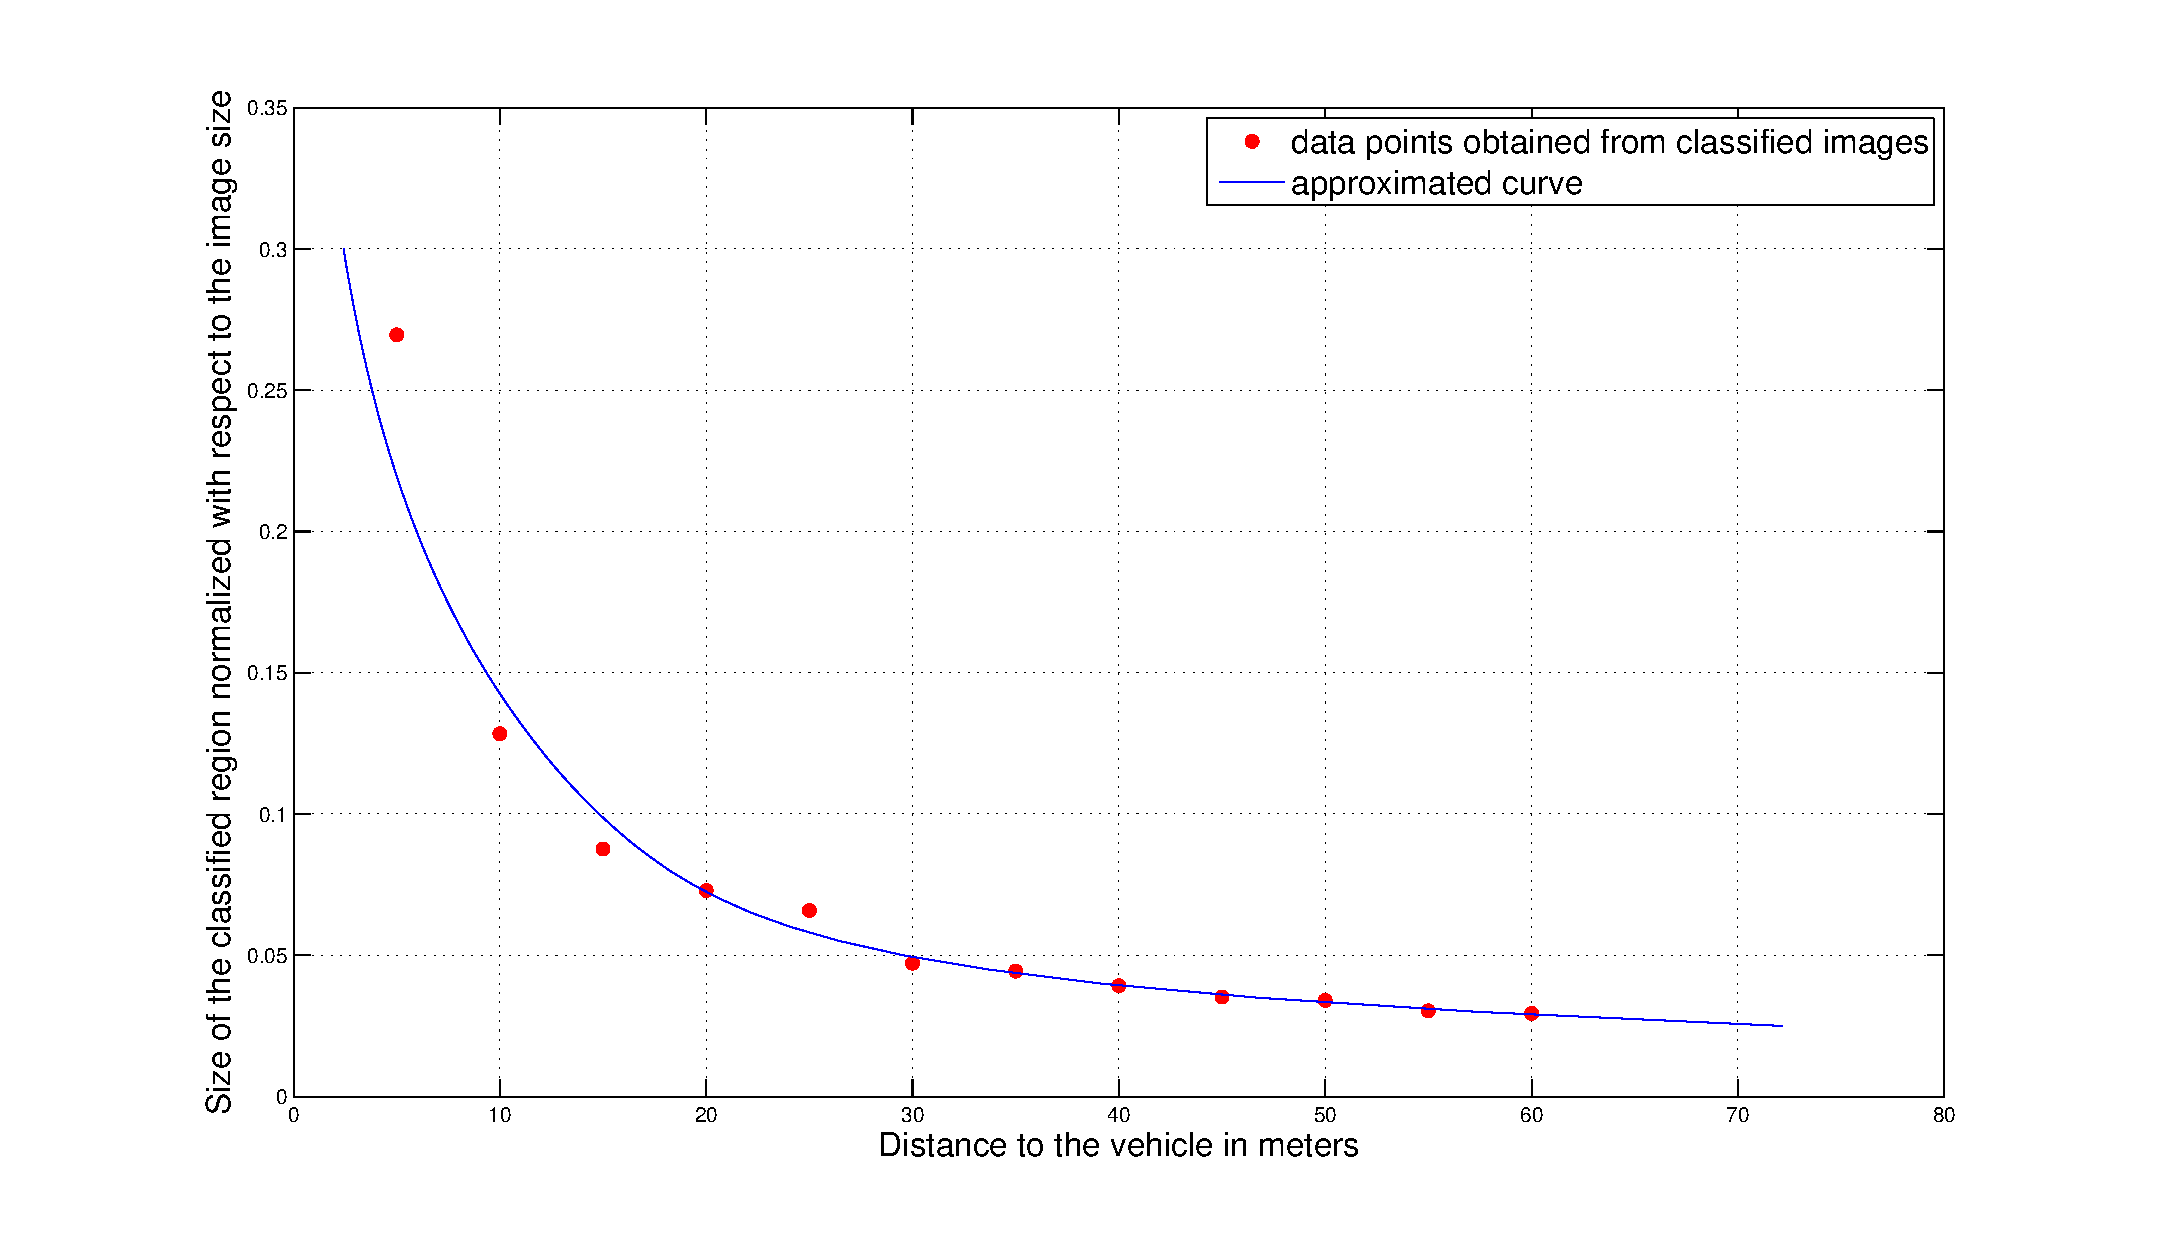
\includegraphics[width=\linewidth]{img/fitted_curve.eps}
\caption{Curve fitting for distance approximation from classification region
    size. In the horizontal axis is the distance to the vehicle in meters.
In the vertical axis is the normalized region size containing the vehicle. The red
points represent the measure obtained from each image. The blue curve is the predicting model fitted to the data points.}
\label{fig:distance-curve-fitting}
\end{figure} 

It is important to point out that this approximated model is directly related to
the classifier itself. This is because the measurements from the pictures are
obtained through it. This implies that whenever the classifier is changed, a new
coefficients are need to be calculated.

In order to do this relation invariant to the image resolution, we normalize the
size in pixels of the region containing the vehicle with the total width of the
image. With this results we find  an approximated distance to the
vehicle, giving an initial solution to the problem of distance estimation.

% section Distance estimation (end)

\section{Vehicle tracking} % (fold)
\label{sec:vehicle-tracking}

Once the classification is done, the estimation of the distance should be
associated to its respective vehicle. For this reason, it is necessary to track
the vehicles appearing in the image. Is obvious that each vehicle has 
a certain motion and position from frame to frame. Ideally, given the
assumptions about the fixed camera view, the motion and position of each
vehicle should be similar between frames.

Traditionally, the \textit{optical flow} is known as the apparent motion of
objects in the image caused by the relative motion of the camera and the scene.
This concept was study in maybe one of the most influential works in computer 
vision done by \cite{lucas-kanade}. In this approach, the image derivatives are
used to obtain a motion vector inside a small windows partitioning the image. 
Later, these velocity vectors can be used with a mean-shift approach to get 
the final position of the object.

In principle, this technique could be used together with the classifier, giving
the last one a starting point for the tracking. This is commonly done because
usually the classification takes more time than the tracking. In this project we
tested this approach by switching between a \textit{detection phase} and a
\textit{tracking phase} periodically. This has proven to be more fast than
performing a detection on each frame.

Now an identification number can be assigned to each vehicle by
thresholding the similarity between the classification regions. Basically, if a 
rectangle appearing in two consequent frames have similar position and size, these
two are consider to correspond to the same vehicle and an identification number
is assigned. 

In figure~\ref{fig:tracking} you can see four sequential images separated by 20
frames in between. The color of the bounding boxes correspond to the identification 
number assigned to a vehicle. For example, the vehicle inside the
yellow box is tracked successfully in the entire sequence. Nevertheless, when a
vehicle is not correctly classified in a particular frame, the tracking is lost.
You can see this in the same figure, the vehicle inside the pink bounding box is 
later labeled with the blue color, meaning that the tracking was lost at some point 
and then rediscovered by the classifier. 

\begin{figure}[t]
\centering
\begin{subfigure}[b]{0.4\textwidth}
\centering
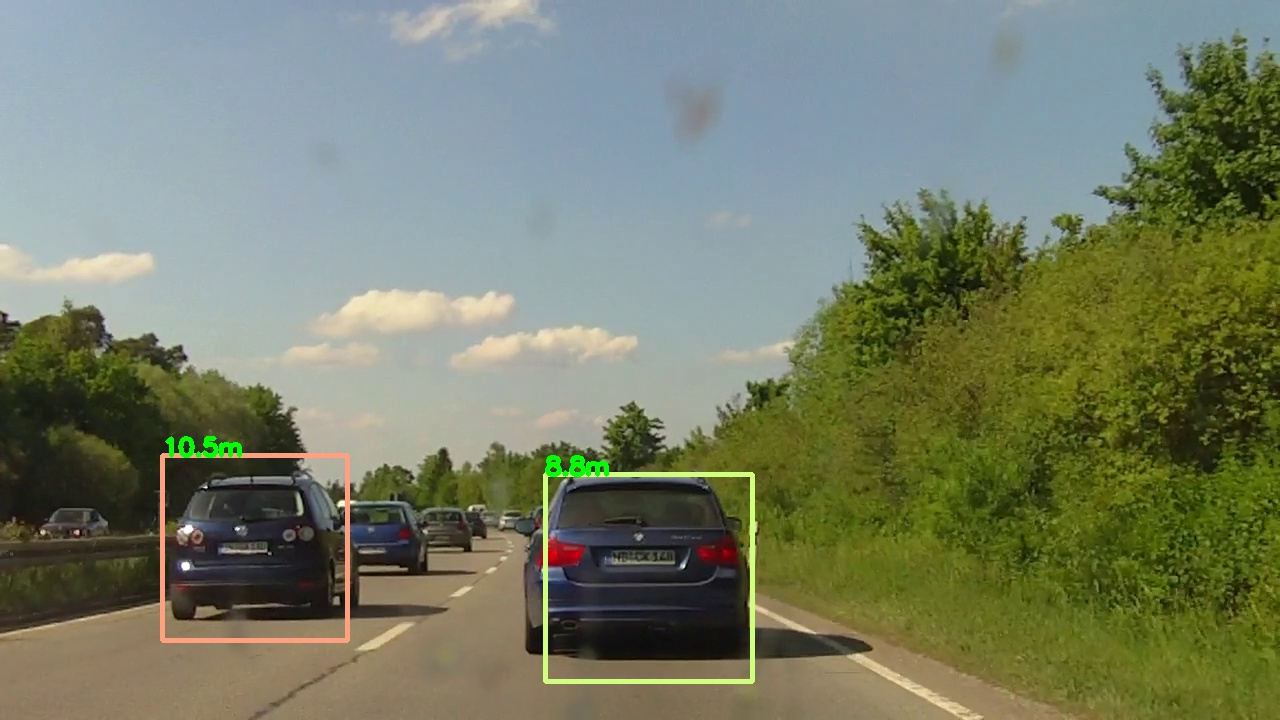
\includegraphics[width=0.9\linewidth]{img/tracking1.jpg}
\vspace{5mm}
\end{subfigure}
\begin{subfigure}[b]{0.4\textwidth}
\centering
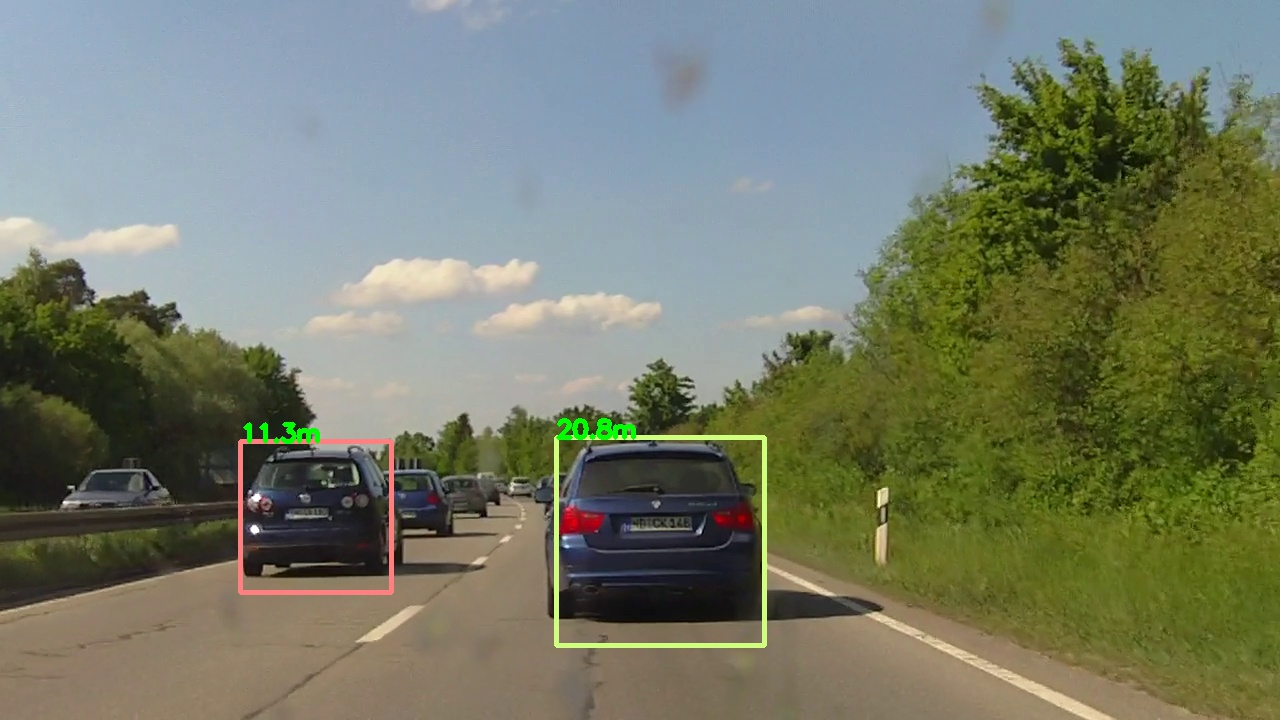
\includegraphics[width=0.9\linewidth]{img/tracking2.jpg}
\vspace{5mm}
\end{subfigure}
\begin{subfigure}[b]{0.4\textwidth}
\centering
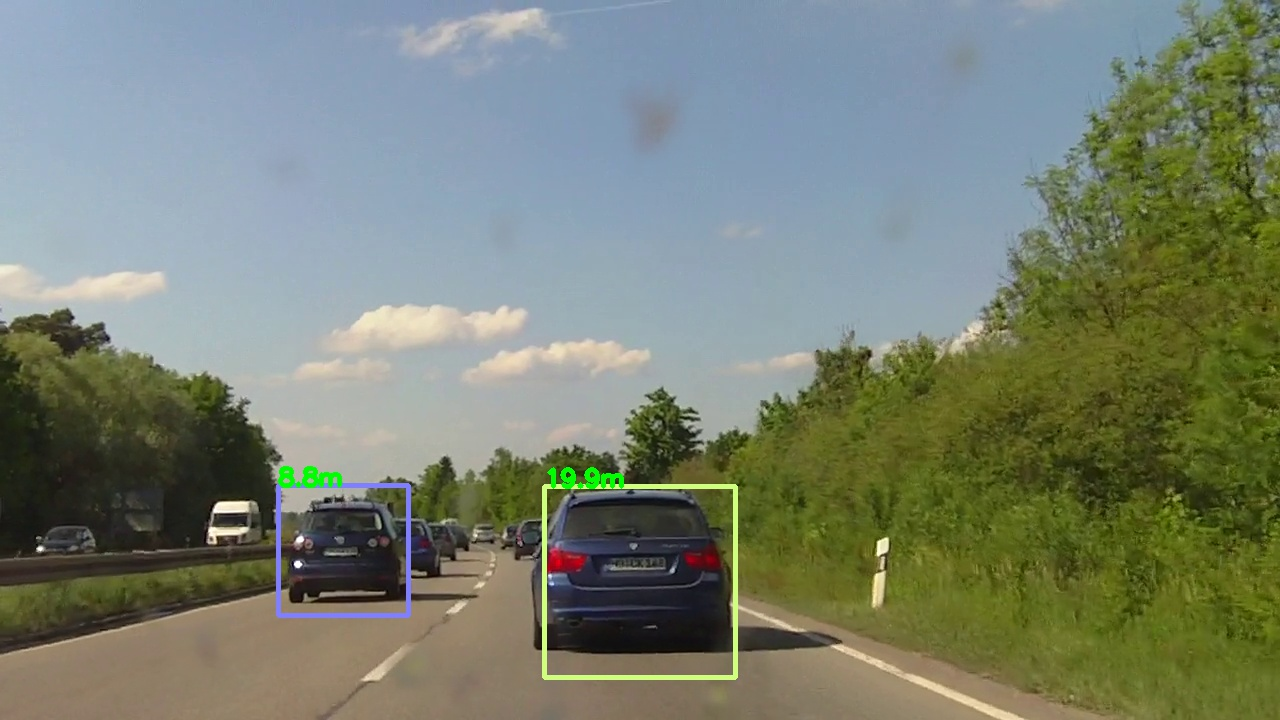
\includegraphics[width=0.9\linewidth]{img/tracking3.jpg}
\end{subfigure}
\begin{subfigure}[b]{0.4\textwidth}
\centering
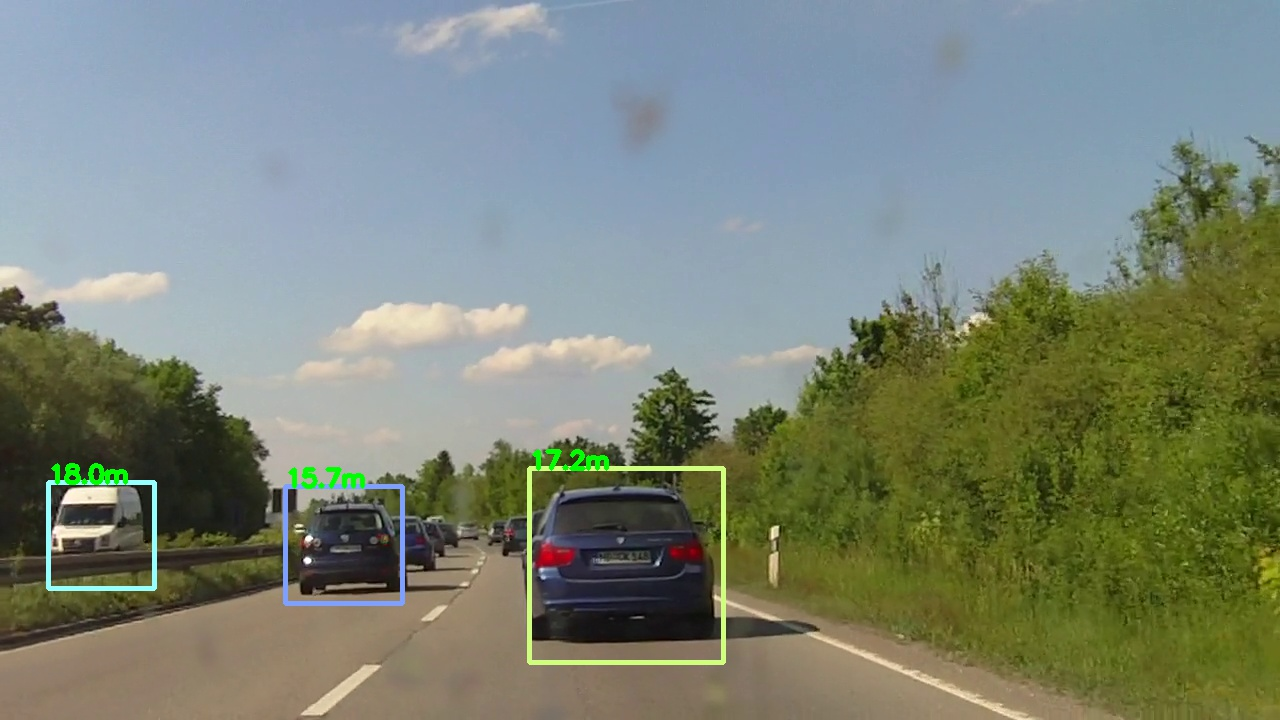
\includegraphics[width=0.9\linewidth]{img/tracking4.jpg}
\end{subfigure}
\caption{Tracking of vehicles. The pictures shown here have 20 frames of
separation.}
\label{fig:tracking}
\end{figure}

% section vehicle-tracking (end)

\section{Speed estimation} % (fold)
\label{sec:speed-estimation}

The missing peace to obtain the metric is to estimate the speed of vehicle with
the on-board camera. In principle for this purpose, the same concept of
\textit{optical flow} explained in the previous section could be applied.
Nevertheless, nowadays is normal that Smart-phones have \textit{Global
Positioning System} or GPS for short. With this technology is possible to
estimate the speed in a more easy and accurate way. This is done by first
estimating the position of the device.

The GPS can estimate the actual position of the device using the received signal
of at least 4 GPS satellites. The distance to each satellite is calculated with
the transit time of the signal and the speed of light. There are other ways to 
calculate position of the device, for example the same idea can also be applied 
to the signal of antennas or even wireless networks access points.

It is trivial to calculate the speed once at least two measured
positions on time are obtained. The strength of this approach lies on the amount of
measurements obtained in time and their accuracy.

% section speed-estimation (end)


\chapter{Implementation and experiments}  
\label{cha:android}

Nowadays the Android operative system is the most popular platform for
Smartphones and mobile devices. Due to this fact, there is a great interest in
the development of all sort of applications and with it, many tools have
been adapted to this platform for the use of the developers. One of these tools
is the OpenCV library for computer vision by \cite{opencv}.

This powerful library have already implemented the most common computer vision
algorithms and methods. In particular we can find the Machine Learning approach
for object detection in images explained in the previous
section~\ref{sec:objectdetec}.  It was perfectly suited by the implementation of this
project.

In this chapter is going to be presented the details about the Android
Application and the qualitative results on the performance of the application.

\section{The Android Application} % (fold)
\label{sec:androidapp}

In this section, the structure of the application is going to be presented. The
functionality of the main components is going to be explained aiming for future
improvements. In the figure~\ref{fig:andrivedir} is illustrated the directory
structure of the application.

\begin{figure}
    \centering\small
    \begin{minipage}[t]{0.6\linewidth}
        \dirtree{%
            .1 Andrive/. 
            .2 jni/. 
            .3 Android.mk. 
            .3 tum\_andrive\_DetectionBasedTracker.h.
            .3 detector\_native\_source.cpp.
            .2 src/. 
            .3 tum/.
            .4 andrive/.
            .5 Andrive.java.
            .5 GPSListener.java.
            .5 DetectionBasedTracker.java.
            .2 res/. 
            .3 raw/. 
            .4 cascade.xml. 
        }
    \end{minipage}
\caption{Directory structure of the Android application}
\label{fig:andrivedir}
\end{figure}

Maybe the most important file is the \textit{cascade.xml}. This file contains
the learned classifier used for image classification and vehicle detection. This
basically implies that it can be easily substituted by any other classifier for
either improving the classification or detect other objects.

Secondly, we have the source files under the \textit{src} directory. For the
vehicle detection module we have basically two files. The
\textit{DetectionBasedTracker.java} which defines the class with the same name.
This class implements the image classification task. It reads the
\textit{cascade.xml} file and use it to classified the images in the way
described in the chapter~\ref{kap:vehicle-detection}. The second file is the
\textit{GPSListener.java} which implements the class in charge of processing the
GPS signal and extract the speed for the calculation of the Time Headway
measurement (THM). 

Finally in the \textit{jni} directory are the native source files used by the
Java Native Interface (JNI). This native source is intended to accelerate the
task of image classification by compiling the methods in the C++ programming
language for the specific architecture. The class \textit{DetectionBasedTracker} 
can call these methods and also their equivalent in the Java programming
language.

The source code of this application can be found in the repository from
\cite{andrive} at GitHub.

% section androidapp (end)

\section{Training the classifier} % (fold)
\label{sec:trainingClasssifier}

In these section is going to be presented the details about the training phase.
The first step is to form the training set. We used a training set combining the
work of Markus Weber and the TME dataset by \cite{tme}. We have gather about 430
positive images and 3000 negative images.

Due to the Adaboost learning algorithm, a proportion of two negative samples for
each positive is recommendable. For this reason, a total number of 1500 positive
images are synthesize form the original 430. The synthesizing process refers to
the process of picking images from the original set of positive samples and
apply light transformations to them. Examples of these transformations are
rotations, light changes and background changes.

Once the dataset is constituted, the images are transformed from the RGB color
space to intensity images. In other words, the images are transformed to gray
scale. The reason is that the classifier can only work on one channel.

The next transformation is to rescale all the images to a size of $20\times20$
pixels. This size represents a trade
of between classification quality and performance speed. The bigger the images,
the more detail on the image structure and better texture description. On the
other hand, the bigger the images, more time the classifier needs to analyse the
entire image.

To train the Adaboost algorithm, it is required to choose 3 parameters, the hit
rate, the maximum false alarm rate and the number of stages. The hit rate is
simply the desired rate of correctly classified examples. In other words, the
hit rate is simply the number of correctly classified examples divided by the
total number of examples. Ideally this rate should be close to 1.0.

The false alarm rate is the number of false positive examples obtained by a
particular weak classifier over the whole dataset. While training, weak
classifiers that have a false alarm rate higher than the maximum specified are
discarded. In practice this threshold should be between 0.45 and 0.5. Remember
that weak classifiers are required just to perform better than random but in
general they can not archive lower false alarm rates by their selves. For this
reason if you specify a very low threshold on the false alarm rate, you get into
the risk of not finding a weak classifier for the actual stage. Finally, the
number of stages refers to the number of weak classifier in the final strong
classifier.

In the figure~\ref{fig:classification-error} is presented the evolution of the
error as new weak classifiers are added to the strong classifier. The error is
measured in the training data and a separate set of data called Testing set,
this final set is composed of examples that are hided from the classifier to
measure its performance on unknown data. As you can see, The more weak
classifiers, the smaller the error on the training set. Nevertheless, notice how
after 16 weak classifiers the performance on the testing set gets worst. This is a
sign that the model is over-fitting the data and it is not generalizing anymore.

\begin{figure}[h]
\centering
\includegraphics[width=\linewidth]{img/classification_error.eps}
\caption{Classification error while training the classifier with respect to the
number of weak classifiers}
\label{fig:classification-error}
\end{figure} 

% section trainingClasssifier (end)

\section{Detection running time} % (fold)
\label{sec:running-time}

In this section is going to be discuss all the factors that directly affect the
running time and the performance of the detection. In the
section~\ref{sec:vehicle-tracking} is explained one of the strategies that can
be implemented to decrease the runing time of the general application. Tracking
an already detected object is faster than performing the detection over the
image. In the figure~\ref{fig:trackingvsdetection} you can see the runing time
in seconds that the detection frame-wise take in comparison with the alternative
of switching between detection and tracking. In average, performing the
detection on each frame takes about 0.2581 seconds while mixing it with the
tracking strategy the average time reduces to 0.0278 sconds.


\begin{figure}[h]
\centering
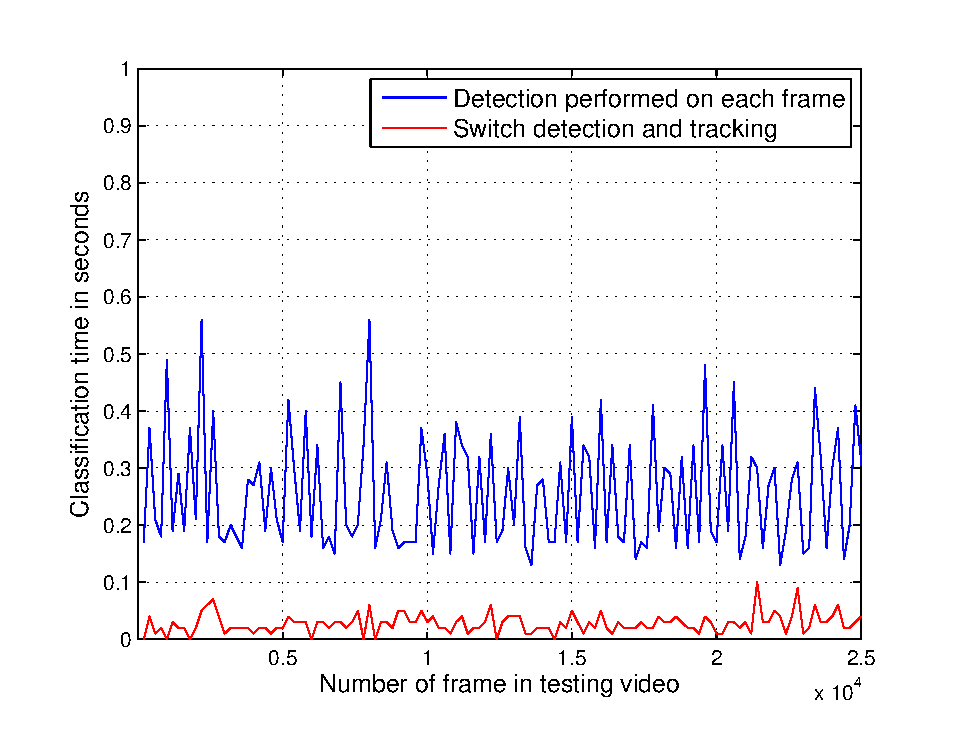
\includegraphics[width=\linewidth]{img/trackingvsdetection.eps}
\caption{Classification time for performing the detection on each
    frame (blue) and switching between detection and tracking (red) along a
    testing video stream}
\label{fig:trackingvsdetection}
\end{figure} 

We test the application on a Samsung S3 GT-I9305 which have a Quad-core 1.4 GHz
Cortex-A9 processor. On the table~\ref{tab:detectionvstracking} are shown the
performance results obtained with the two methods and the average frames per
second using both approaches. Using the mixed strategy push up the frame rate
almost four times.
 
\begin{table}
\begin{tabular}{|c|c|c|c|}
    \hline
    Method & Average running time (sec) & variance & Average FPS \\
    \hline
    Frame-wise detection & $0.1746$ & $7.224 \times 10^4$ & $5.8838$ \\
    \hline
    Detection and tracking  & $0.0555$ & $6.3127 \times 10^5$ & $18.36$ \\
    \hline
\end{tabular}
    \caption{Performance comparison between pure detection and switching between
    detection and tracking}
    \label{tab:detectionvstracking}
\end{table}

An other important comment is that the code was implemented on C++ and executed
by the Android NDK interface. The native code in C++ runs much faster than its
Java counterpart.

% section Performance and running time (end)




\chapter{Lane Detection, Tracking and SDLP Calculation}  \label{kap:sdlp}

Everybody in this world is concerned about safety. The people those who go out from
one place to other, expect to reach safely. Without any sudden incidents which may come 
through externally by road accidents while travelling. We can avoid the road accidents by 
using improved driving assistances. Therefore, a system that provides a means of warning 
the driver to the danger has the potential to save a considerable number of lives. One of the 
main technologies involved in these tasks is computer vision, which become a powerful tool for 
sensing the environment and detect road boundaries. Lane detection and object detection plays 
vital role for accidents. For human vision and human intelligence the task of lane detection and 
object detection changes due to variations in the road conditions. Sometimes it is very easy to 
detect with the human eyes but in some conditions due to externals effects the human intelligent 
have detection problems. 

Driver inattention has been a major focus of driver safety research (Klauer et al., 2006; 
Ranney et al., 2000; Wang et al.,1996). In recent years however, naturalistic studies have made 
it possible to gain additional insights on driver behavior and have actually demonstrated that 
78\% of crashes and 65\% of near crashes are driver inattention related (Klauer et al., 2006). The 
main causes of collisions can be driver error, drowsiness, impaired driving due to alcohol/drugs 
or distractions due to a phone call or tuning the radio. Many studies have shown that driver 
inattention can influence lane-keeping ability. One of the main source of making this analysis on 
vehicle control is the standard deviation of lateral position (SDLP), ie, the
amount of ``weaving''
of the car.

The basic purpose of developing this android app as a proof of concept is to help
researchers in domain of ergonomics to investigate driver's behavior in different scenarios. We 
are proposing a system which acquires the front view using an android phone camera mounted 
on the vehicle then applying few processes in order to detect the lanes. We are using an open 
source code for lane detection \cite{lane-code} to provide the baseline functionality which is developed to run 
on PC. Code is ported to Android NDK project and then improved further and features added as 
per our requirement.

\section{Lane Detection and Tracking}

Lane departure warning system is a mechanism designed to warn a driver when the 
vehicle begins to move out of his lane (unless a turn signal is on in that
direction) on freeways and arterial roads. Lane detection algorithms detect lane markings and the edges
of the road, and estimate the vehicle position in the lane. A lane detection system must be
able to pick out all manner of markings from cluttered roadways and filter them to produce a
reliable estimate of the vehicle position and trajectory relative to the lane.

A typical lane tracking process includes:

\begin{itemize}
    \item Video acquisition.
    \item Matrix downsampling and set Region of Interest (ROI).
    \item Line Detection.
    \item Lane Detection.
    \item Lane Tracking.
\end{itemize}

\begin{figure}
\begin{center}
    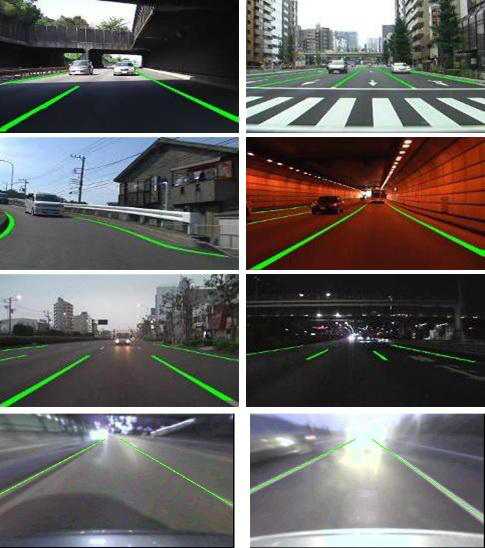
\includegraphics[scale=0.6]{img/lane1.png}
\end{center}
\caption{Examples of lane detection and tracking}
\label{fig:lane1}
\end{figure}

We are using some assumptions for our solution as it is a prototype and also we
something which is manageable but still suffice the need of a good proof of concept. 

\begin{itemize}
\item Road is assumed to be of fixed lane width and constant texture so that
searching for parallel lane markings is efficient.
\item It is a constraint to process the varying painted and the unpainted roads or
the dash and the solid paint line roads. Its good to assume a continuous or dashed but bright
lane markings.
\item It is a constraint to handle the curved roads and good assumption is that the
roads are straight without intersections and bumps.
\item Experimental results are not constraint to be robust against noise, shadows
due to trees/ building, and illumination variations in the captured road images. Other issues
are due to wet road, direct sunshine on the cameras, tunnels and bridges' shadows.
Avoidance of these possibilities simplifies road geometry reconstruction. 
\item Other vehicles on the path partly occlude the visibility of the road and
    therefore also of road markings. The road is assumed to be one way but can by 2 lane road.
\item A constant weather and lighting conditions are assumed. More precise, the 
    video stream that will be used for training and testing are going to be taken 
    during daylight and without rain or fog.
\end{itemize}

\subsection{Video acquisition}

There are many sources for the video acquisition in field of signal processing.
The main important one is vision based approach. In our project, we are using
Android phone camera instead of an external camera and video stream recorded by camera would
be used as input. Now we have really powerful android phones with normally 5 MP camera
which is good enough for Computer Vision applications. In our case, phone is mounted on the
dashboard in a landscape position where it can get a good view of the road surface and the
vanishing point of road should be somewhere at center.

\subsection{Matrix downsampling, Grey scaling and setting Region of Interest (ROI)}

Computation of Image processing algorithms is very resource oriented task on
Smartphones but there are several proven techniques which can be used to limit
the enormous space of frames in which each window has to pass the classifier. Otherwise we
were facing extremely poor frames per second (fps) rate. 

One of the techniques is to downsample the matrix by reducing the size of image
frame.  It reduces quality which is a tradeoff but it doesn't affect significantly on
ultimate output. We are reducing the size of each input frame by 1/4 and then upsampling it again by
factor of 4 before displaying it back on screen. This concept is also referred as Scale Space.

\begin{figure}
\begin{center}
    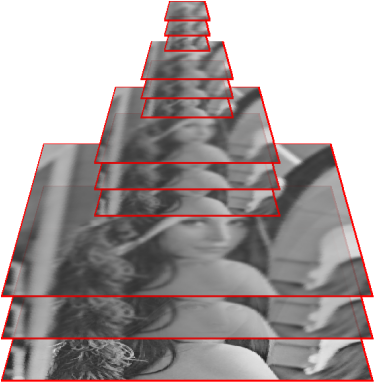
\includegraphics[scale=0.6]{img/lane2.png}
\end{center}
\caption{Scale Space Demonstration}
\label{fig:lane2}
\end{figure}

The captured image is also converted to gray scale to make method faster, less
computations, and less sensitive to scene condition \cite{lane2}. The other influential
technique is setting a custom Region of Interest (ROI) to limit the search for
lane markers to a specific region of the image to speed things up. This helps in
segmentation of the space and remove all areas that we are certain of not
containing the lane markings. It creates a binary mask and only detect in
windows that lie in the smallest bounding box of our blobs of possible
candidates.

\begin{figure}
\begin{center}
    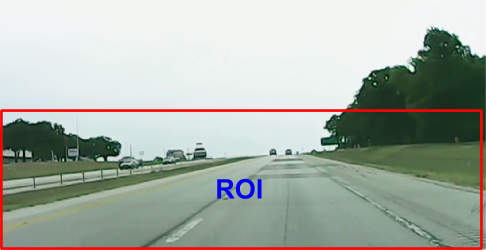
\includegraphics[scale=0.6]{img/lane3.png}
\end{center}
\caption{Region of Interest selection}
\label{fig:lane3}
\end{figure}

\subsection{Canny Edge Detection}

Canny edge detection is one of the edge detection methods that is used to find all the edge points in the image and output is a binary map. Canny runs a gradient on the image to find sharp changes in the pixel intensities. These are likely contours in the image. The output is then just a binary map that shows you where the contours of the image are located. 

In this step, we use Canny edge detection to find lane boundaries in the frame. Canny edge detection basically uses gradient vector of an intensity image. Lane boundaries have high contrast in the image, and this feature yields high values of gradient vector by which we can find the edge direction, which is orthogonal to gradient vector. It is one of the best and efficient methods among many edge detection methods \cite{lane3}.

\begin{figure}
\begin{center}
    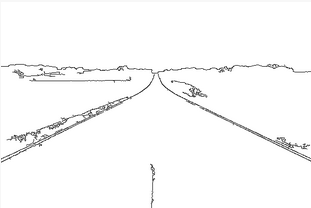
\includegraphics[scale=0.6]{img/lane4.png}
\end{center}
\caption{Example of a contour image}
\label{fig:lane4}
\end{figure}

\subsection{Hough Transform}

The Hough transform is a technique which can be used to isolate features of a particular shape within an image. Developed by Paul Hough in 1962 and patented by IBM, the transform requires the desired features to be specified in some parametric form, the classical Hough transform is most commonly used for the detection of regular curves such as lines, circles, ellipses, etc. The main advantage of the Hough transform technique is that it is tolerant of gaps in feature boundary descriptions and is relatively unaffected by image noise.

Let's take an image (figure~\ref{fig:lane5}) with two lines A and B. Obviously both lines are each made of its own set of pixels laying on a straight line. Now, one way or another we need to learn our software which pixels are on a straight line and, if so, to what line they belong to.

\begin{figure}
\begin{center}
    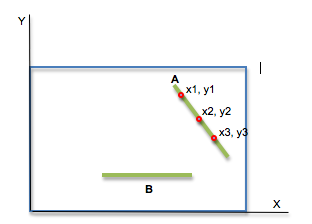
\includegraphics[scale=0.6]{img/lane5.png}
\end{center}
\caption{Line creation from points.}
\label{fig:lane5}
\end{figure}

\begin{figure}
\begin{center}
    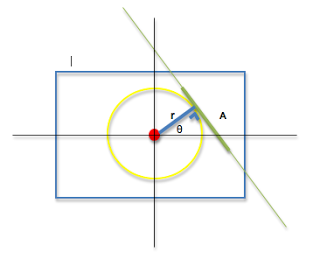
\includegraphics[scale=0.6]{img/lane6.png}
\end{center}
\caption{The transformation.}
\label{fig:lane6}
\end{figure}

The trick of the Hough Transformation is to represent lines in a polar coordinate system (see figure~\ref{fig:lane6}), or in this case, also called "Hough Space". 

The important thing in figure~\ref{fig:lane6} is that we imagine a line from the center (the blue line) which is perpendicular to the line we want to find (the green line) and we call the distance from the center $r$ and $\theta$(theta) is the angle to the $X$ axis (the angle between the blue line and the $X$ axis).

The transformation from any $(x, y)$ pixel in figure~\ref{fig:lane1} to the $(r, \theta)$ representation in figure~\ref{fig:lane6} is the following:

\begin{equation}
    r = x \cos(\theta) + y \sin(\theta) 
\end{equation}

Now, if you lean back and think a bit about Fig 6. Every possible line can be represented by a unique $r$ and $\theta$. And further, every pixel on a given line will transform to the exact same $r$ and $\theta$ for that line. And this is immediately the most important aspect of the whole Hough stuff. 

\subsection{Lane Detection}

Lane detection phase uses the Hough Lines function to extract line segments in the image based on Hough transform. The parameters are thresholded version of contours, the Hough Lines which become the output and the Hough Vote. The Hough Vote is an important parameter because it influence the accuracy and time taken by the algorithm. It is basically the minimum number of points passing through a line. So the higher value of Hough Vote means the smaller inaccurate lines would be rejected and helps in removing the noise but the trade-off is performance. We have added a slider input ( 0 - 200 ) before the start of the application instead of making it fixed so that user can change Hough Vote value which can help in investigation of the researcher.

The Hough Lines object finds Cartesian coordinates of lines that are described by rho and theta pairs. The lines are filtered on basis of theta and lines with theta values between 4 degrees and 84 degrees or between 95 degrees and 180 degrees are allowed only to pass through. This is to ensure that we have the lines which are more probably the true lanes. Then we want to find the point of intersection i.e\ $x$ and $y$ so that we can plot the line by connecting these points.

\begin{equation}
    x = \frac{r - y\sin(\theta)}{\cos(\theta)} \hspace{1cm} y = \frac{r - x
    \cos(\theta)}{\sin(\theta)}
\end{equation}

\begin{figure}
\begin{center}
    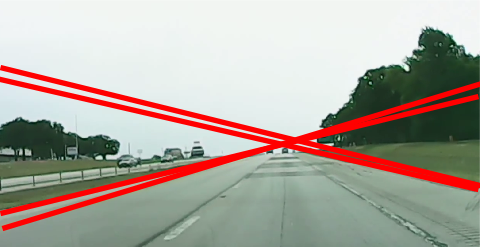
\includegraphics[scale=0.6]{img/lane7.png}
\end{center}
\caption{After applying Hough Transform and Hough Lines}
\label{fig:lane7}
\end{figure}

The problem with this current progress is that we can not find the endpoints of the lane that is also known as vanishing point of lane. For this, Probabilistic Hough Transform \cite{lane4} is used which is pretty much the same as regular Hough Transform but finds the end of each line as shown in the diagram below.


\begin{figure}
\begin{center}
    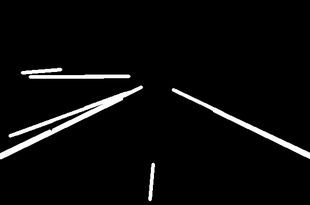
\includegraphics[scale=0.6]{img/lane8.png}
\end{center}
\caption{shows the output of Probabilistic Hough Transform with end points of lane}
\label{fig:lane8}
\end{figure}

The regular transform does not find endpoints and the probabilistic tends to find several other lines that is not required. To solve this problem, a bitwise addition of two images is done. The final output looks like the image below.

\begin{figure}
\begin{center}
    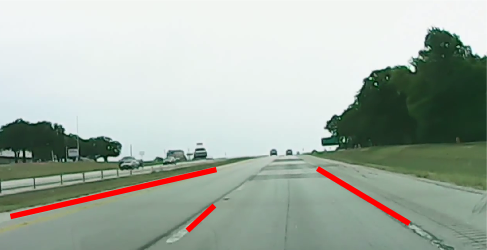
\includegraphics[scale=0.6]{img/lane9.png}
\end{center}
\caption{Shows final output after bitwise addition}
\label{fig:lane9}
\end{figure}

\section{SDLP calculation and Ergonomics}

Our project aims is to develop an android app which will help researchers in investigating and evaluating different driving behaviors in different situations from ergonomics perspective. Many studies have shown that driver inattention can influence lane-keeping ability and hence road accidents. Ergonomics researchers intent to investigate how the car interior can be a reason to distract driver and cause inattention with eyes-off-road. Research has shown that after accounting for driving speed and lane width, the eyes-off-road significantly increased the standard deviation of lane position (SDLP). Visual related distractions occur when drivers need to divert their eyes away from the roadway such as when texting, tuning radio, selecting the playlist etc. 

SDLP stands for standard deviation of lateral position and is considered the primary outcome measure of vehicle control. The secondary outcome measure is the standard deviation of speed (SDS). Since SDLP increment may ultimately result in lane crossings into the road shoulder and adjacent traffic lane, it can also be regarded as a potential index of driving safety. It is considered an international standard of evaluation in the on-the-road driving test around the globe. 


\begin{figure}
\begin{center}
    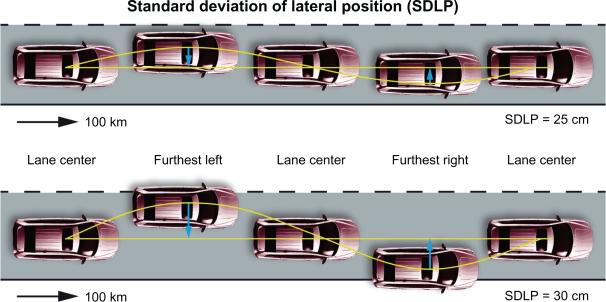
\includegraphics[scale=0.6]{img/lane10.png}
\end{center}
\caption{SDLP demonstrated}
\label{fig:lane10}
\end{figure}

\subsection{Lateral position estimation}

Lateral position refers to the relationship of the correct position of car in lane to a real position of car in the lane. The difference between the true position of car and the actual position of car in lane gives an understanding of how much is driver deviating. This can be directly computed from the distance between the vehicle and the lane marker under the assumption of a fixed lane width (3.56 m) and a known vehicle width (1.52 m). 

In our case, car's position is equivalent to the value of $x$ coordinate of the line detected in the final output. We have defined a scale of values ranging from 450 to 100 for our test video which involves single lane. The selection of this video has many reasons for training and testing. It involves lane switching of driver, there are very few cars on road, the lane boundaries are pretty clear without any shadows and the video is made in daytime so there's enough light. During the training phase, the scale was defined for both lanes. The hypothesis used is that the lanes which are visible in the smartphone camera view actually define the position of car in the lane. Thats why SDLP in our case is just an estimate. 

\subsection{Calculating SDLP}

formula, table of values, results, graphs

The SDLP is calculated the following way:

\begin{itemize}
    \item Calculate the mean lateral position (MLP) for the entire drive 
    \item Calculate the standard deviation of the MLP (= SDLP) across all of the samples taken
\end{itemize}

The equation to calculate a standard deviation is:
When $X$ is the lateral position (determined for each valid data point) with a
mean value $\mu$:

\begin{equation}
    MLP[X] = \mu
    \label{eq:lane1}
\end{equation}

In equation~\ref{eq:lane1}, MLP (mean lateral position) denotes the average of
$X$. The standard deviation of $X$ is the quantity:

\begin{equation}
    SLDP = \sqrt{MLP[(X - \mu)^2]}
\end{equation}

In other words, SDLP is the square root of the variance of $X$, i.e., it is the
square root of the average value of $(X - \mu)^2$.

The following graph shows average values of SDLP calculated from a demo video. The mean value is around 0.80 which is a poor estimation and the reason is that boundary detection is sometimes very inaccurate. The noise data has a negative impact on the dataset. 


\begin{figure}
\begin{center}
    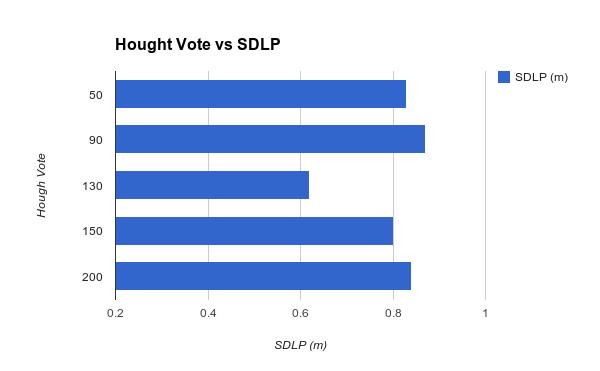
\includegraphics[scale=0.6]{img/lane11.png}
\end{center}
\label{fig:lane11}
\end{figure}

\section{Implementation and Evaluation}

For implementing this proof of concept, we are using Android SDK and Android NDK platform. For computer vision operations, OpenCV Library is used and languages include Java and C++. 

Project Structure :-

\begin{figure}
    \centering\small
    \begin{minipage}[t]{\linewidth}
        \dirtree{%
            .1 Application/.
            .2 jni : Conventional location for C/C++ source code.
            .3 Android.mk : sub-makefile that describes the C++ static libraries and *.so files.
            .3 Application.mk : contains settings that apply to all the C/C++ code.
            .3 LaneDetector.cpp : main cpp file that handles everything.
            .3 linefinder.h : class file that implements lane detection functions.
            .3 LaneCalculations.cpp : implements sdlp functions.
            .3 LaneCalculations.h : class file for sdlp functions.
            .2 res : Conventional location for Android XML resource files.
            .3 src : Conventional location for Android Java source code.
            .3 tum.andrive.lanedetection.
            .4 LaneDetector.java : Main java file.
            .4 VerticalSliderActivity.java : java file to display and process slide.
            .2 AndroidManifest.xml : Specifies App's icon, required Android version, and a list of all activities.
        }
    \end{minipage}
\end{figure}

\subsection{Android NDK}

Vision processing algorithms were originally only capable of being implemented on costly, bulky, and power-hungry high-end computers. As a result, computer vision has historically been primarily confined to a scant few application areas such as factory automation and military equipment. The raw computing power in the modern-day mobile smartphone and tablet is now at the point where the implementation of embedded vision is not just possible but practical.

The OpenCV (Open Source Computer Vision) Library was created to provide a common resource for diverse computer vision applications and to accelerate the use of computer vision in everyday products \cite{lane5}. OpenCV4Android is the official name of the Android port of the OpenCV library. There are normally 2 ways to implement Computer Vision apps in Android. One is using the OpenCV Java API and other one is using native C++ to write the OpenCV portion of application. 

Both approaches uses the Java wrapper and there is a performance penalty on every OpenCV function called per frame. When using the Java API, for example application calls three OpenCV functions per video frame so this particular application will incur six total JNI call penalties per frame as per shown in Fig. A slightly more difficult but more performance optimized development method uses the Android NDK (Native Development Kit). In this approach, the OpenCV vision pipeline code is written entirely in C++, with direct calls to OpenCV. You simply encapsulate all of the OpenCV calls in a single C++ class, calling it once per frame as shown in Fig. With this method, only two JNI call penalties are incurred per frame, so the per-frame JNI performance penalty is significantly reduced. Java is still used for non-vision portions of the application, including the GUI. We are using the second approach to follow an optimized path. 


\begin{figure}[t]
\begin{subfigure}[b]{0.5\textwidth}
\centering
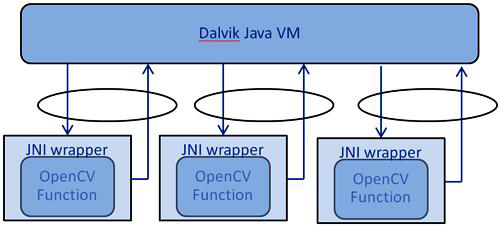
\includegraphics[width=0.85\linewidth]{img/lane12.png}
\caption{When using the Java API}
\label{fig:lane12}
\end{subfigure}
\begin{subfigure}[b]{0.5\textwidth}
\centering
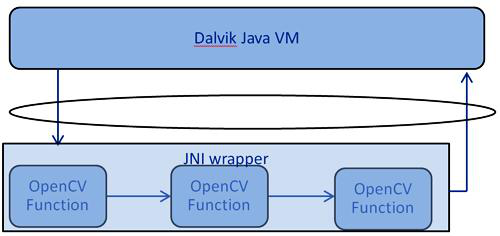
\includegraphics[width=0.85\linewidth]{img/lane13.png}
\caption{Using native C++ to write functions}
\label{fig:lane13}
\end{subfigure}
\end{figure}

\subsection{Class Structure}

Class diagrams represent the structure of classes used in the source code. LineFinder class represent the class which implements the major lane detection and over-laying functions. LaneCalculation class represent functions which are used to calculate lateral position and SDLP values.

\begin{figure}
\begin{center}
    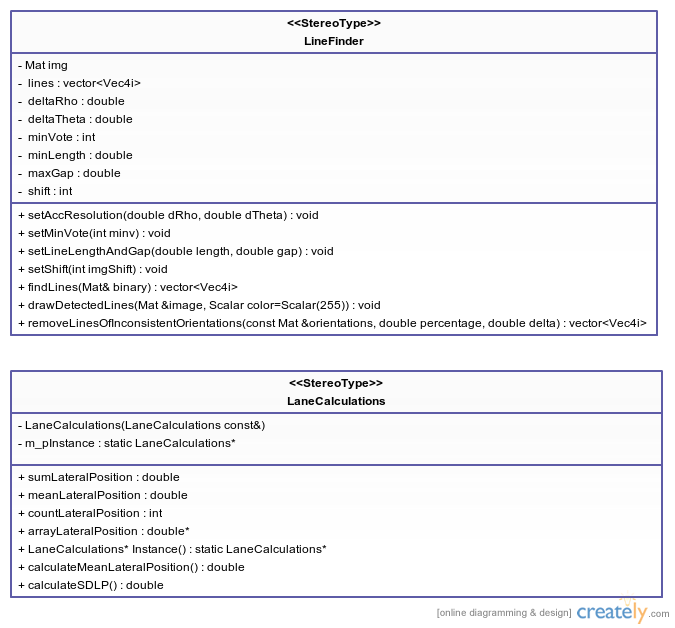
\includegraphics[scale=0.6]{img/lane14.png}
\end{center}
\caption{Class diagrams of main classes}
\end{figure}

\subsection{Optimization and Contributions}

My contribution to the original open source code and optimization techniques which were applied includes :

\begin{itemize}
        \item Creating an Android app, porting the desktop code and customizing it to run on Android NDK
        \item Getting camera input from Android phone in an efficient way using CameraBridgeViewBase class [ref]
        \item Downsampling the input frame by 1/4 before applying computations and then upsampling again before passing it back to JNI wrapper
        \item Using Region of Interest (ROI) by applying a mask and fetching only required area of input and not the whole frame
        \item Adding additional flags in Android.mk and Application.mk files which are used to specify information to Android NDK application
\end{itemize}

I have tested the app on Samsung S5 which is a high-end android phone with quad-core processor. The test case used is the youtube video [6] which is also mentioned previously in the document. Values of Hough Vote were changed using the slider and then once run, frame per second (fps) value is displayed on top left corner of screen. I have used only landscape mode because portrait mode limits the view and we need a good horizontal view of the road. The bar chart shown below shows that fps readings improved significantly after optimization although they are still not very good. The Hough Transform algorithms are very resource intensive. 

\begin{figure}
\begin{center}
    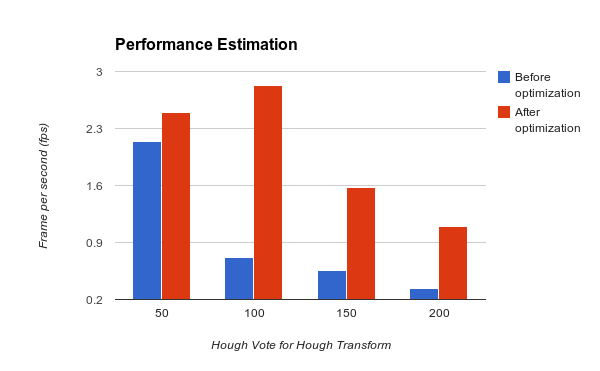
\includegraphics[scale=0.6]{img/lane15.png}
\end{center}
\caption{Class diagrams of main classes}
\end{figure}

\subsection{Issues and Improvements}

This project was a basic prototype or proof of concept developed with many assumptions and certain compromises were made. This is definitely not state-of-the-art solution but can be further used and improved to achieve better results. 

\begin{itemize}
        \item More advanced and better techniques can be incorporated for rapid automated detection of lane boundaries and more accurate overlaying
        \item A technique which can also detect curvatures on lane accurately
        \item A better visualization of lane boundaries and the region in focus to help driver in better understanding of his lane
        \item Improve performance of the app and achieve higher frame per second (fps) rate
\end{itemize}

\subsection{Licenses}

This program is free software; permission is hereby granted to use, copy, modify, and distribute this source code, or portions thereof, for any purpose, without fee, subject to the restriction that the copyright notice may not be removed or altered from any source or altered source distribution. The software is released on an as-is basis and without any warranties of any kind.    In particular, the software is not guaranteed to be fault-tolerant or free from failure. The author disclaims all warranties with regard to this software, any use, and any consequent failure, is purely the responsibility of the user.


% %ERGEBNISSE

\chapter{Bibtex, Citavi und Zitieren} \label{kap:bibtex}
Diese LaTeX-Vorlage verwendet Bibtex zur einfachen Darstellung eines Literaturverzeichnisses.

Es gibt verschiedene Editoren f�r Bibtex Dateien, z.B. JabRef.

Wird mit Citavi gearbeitet, so kann die Literatur automatisch in eine Bibtex-Datei geschrieben werden. \\

Daf�r auf Datei -> Exportieren

\begin{figure}[h]
	\centering
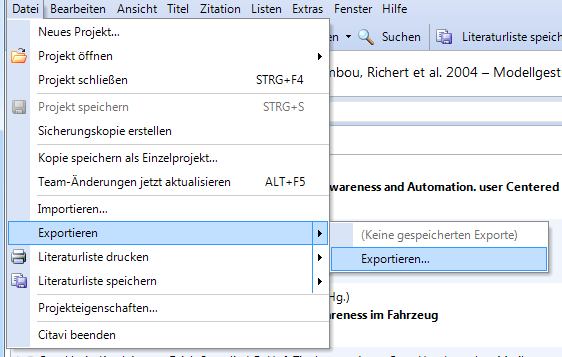
\includegraphics[width=12cm]{img/bib1.png}
\caption{\textit{Exportieren}}
\label{fig:bib1}
\end{figure} 

Im n�chsten Fenster auf "Alle XX Titel in diesem Projekt" und "Weiter".\\

Anschlie�end "BibTeX" anw�hlen und "Weiter".

\begin{figure}[!ht]
	\centering
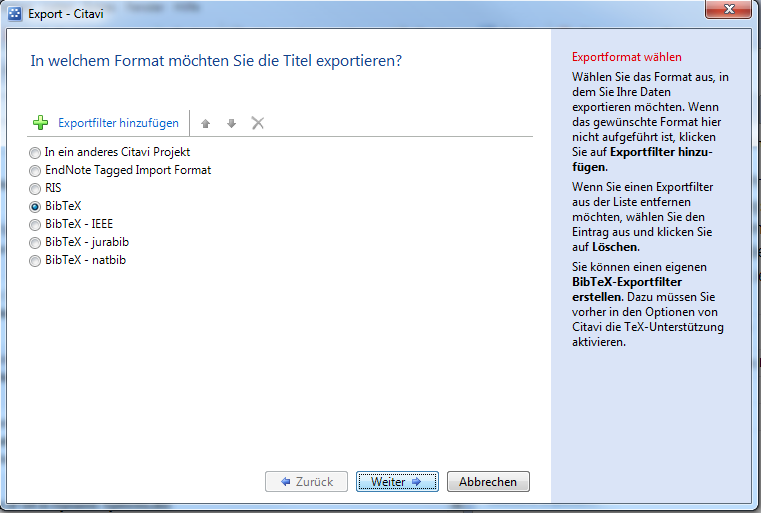
\includegraphics[width=13cm]{img/bib2.png}
\caption{\textit{Fomart zum Exportieren}}
\label{fig:bib2}
\end{figure} 

Jetzt die entsprechende *.bib Datei ausw�hlen. Diese sollte in dem Projektordner liegen und Bibtex.bib hei�en. F�r einen anderen Ort oder Dateinamen muss "$\backslash$bibliography\{Bibtex\}" im "Studienarbeit.tex" entsprechend angepasst werden.
Au�erdem einen Haken bei "Bibtex-Datei aktualisieren".

\begin{figure}[!ht]
	\centering
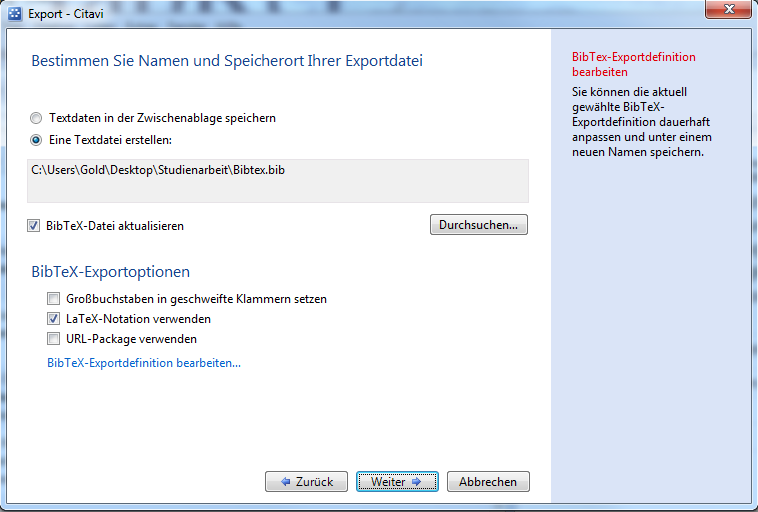
\includegraphics[width=13cm]{img/bib3.png}
\caption{\textit{Datei ausw�hlen}}
\label{fig:bib3}
\end{figure} 

Im n�chsten Fenster der Exportvorlage einen Namen geben und einen Haken bei "Automatisch exportieren beim Speichern" setzen. 

\begin{figure}[ht]
	\centering
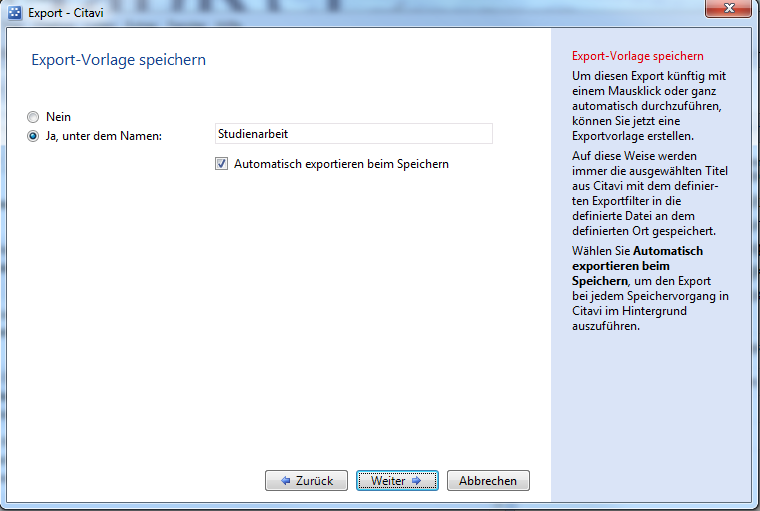
\includegraphics[width=13cm]{img/bib4.png}
\caption{\textit{Automatisch aktualisieren}}
\label{fig:bib4}
\end{figure} 

Bei jeder �nderung in Citavi aktualisiert sich die Bibtex-Datei automatisch mit und ist somit immer auf dem aktuellstem Stand. 

Die gesamte in Citavi gespeicherte Literatur steht nun zum zitieren bereit und es kann mit "$\backslash$cite\{Name.Jahr\}" eine Literaturangabe gesetzt werden. Damit alle Zitate und Seitenzahlen stimmen, muss das Projekt am Ende mehrfach kompiliert werden.\\

Beispiel:

So sagte \cite{Mustermann.2012}, dass... bzw. "Ich bin klug" \citep{Mustermann.2012}.





% --------------------------------------------------
% -------------- LITERATURVERZEICHNIS --------------
% --------------------------------------------------
	
	
\bibliographystyle{apalike} %Zitierstil wie APA6
\bibliography{Bibtex} %Bibliotheksdatei, hier Bibtex.bib



% --------------------------------------------------
% ------------------ VERZEICHNISSE -----------------
% --------------------------------------------------


\listoffigures %Abbildungsverteichnis
\listoftables %Tabellenverzeichnis



% --------------------------------------------------
% --------------------- GOSSAR ---------------------
% --------------------------------------------------


%Sollte ein Glossar erw�nscht sein:
\addcontentsline{toc}{chapter}{Glossar}
\chapter*{Glossar}
\begin{tabbing}
\hspace{3cm} \= \hspace{10cm} \kill \\
MfG \> Mit freundlichen Gr��en\\
\end{tabbing}
 %Bitte bearbeiten




% --------------------------------------------------
% -------------------- ANHANG ----------------------
% --------------------------------------------------


\begin{appendix} %Anhang
\refstepcounter{chapter}
\addchap{Anhang}
Anhang A 

\end{appendix}

\end{document}

% --------------------------------------------------
% --------------------------------------------------
% --------------------------------------------------
